% создаем документ типа "отчет"
\documentclass[a4paper,12pt]{report}
% фишки для набора формул
\usepackage{amsmath,amssymb}
% размер формул
%\DeclareMathSizes{12}{12}{10}{8}
% для вывода русских символов задаем шрифты и кодировки
\usepackage[T1]{fontenc}
\usepackage[utf8x]{inputenc}
\usepackage[russian]{babel}
\usepackage{pscyr}
% рулим полями страницы
\usepackage[top=2cm, bottom=2cm, left=2cm, right=1.5cm]{geometry}
% включаем возможность создания длинных таблиц, которые находятся на нескольких листах
\usepackage{longtable}
% рулим header-ами и footer-ами
\usepackage{fancyhdr}
% включаем возможность copy-paste из PDF
\usepackage{cmap}
% для абзацных отступов (красная строка)
\usepackage{indentfirst}
% в России после номера таблицы ставится точка, а не двоеточие, поэтому нужен этот пакет
\usepackage[font=footnotesize,labelsep=period,skip=0pt,singlelinecheck=false,center]{caption}
% нужно для ввода в таблицы инструкции m{..} - позволяет центрировать по вертикали содержимое ячеек
\usepackage{array}
% нужно для аналогов rowspan в HTML
\usepackage{multirow}
% косая черта в ячейке таблицы
\usepackage{slashbox}
% ссылки в тексте документа
\usepackage[colorlinks,filecolor=black,citecolor=black,linkcolor=black,unicode]{hyperref}
% вставка рисунков
\usepackage{graphicx}
% относительный путь до каталога с рисунками
\graphicspath{{img/}}

\bibliographystyle{unsrt} % стиль библиографических ссылок БибТеХа

\newcommand{\docTitle}{Методы оптимизации}
\newcommand{\docVersion}{0.1}
\newcommand{\HRule}{\rule{\linewidth}{0.5mm}} % своя команда для рисования линий на титульной странице

\renewcommand{\theenumi}{\arabic{enumi}} % меняем везде перечисления на цифра.цифра
\renewcommand{\baselinestretch}{1.25} % делаем полуторный интервал

% переопределяем стиль страницы с собственными header-ами и footer-ами
\fancypagestyle{plain}
{
  \lhead{\textbf{\docTitle} (текст лекций)} % слева в header-е название документа
  \chead{}
  \rhead{\emph{Версия:} \docVersion} % справа в header-е номер версии
  \lfoot{}
  \cfoot{}
  \rfoot{\thepage} % справа в footer-е номер страницы
  \renewcommand{\headrulewidth}{0.4pt} % отчеркивание для header-а
  \renewcommand{\footrulewidth}{0.4pt} % отчеркивание для footer-а
}

\begin{document}

\begin{titlepage}

\begin{center}

% Разработчик
\textsc{\LARGE Прудников А.М.}\\[7.0cm]

% Общий заголовок
\textsc{\Large Текст лекций по курсу}\\[0.5cm]

% Заголовок конкретного документа
\HRule \\[0.4cm]
{ \huge \bfseries \docTitle}\\[0.4cm]

\HRule \\[1.5cm]

% Редакция
\begin{minipage}{0.8\textwidth}
\begin{flushright} \large
\emph{Версия:} \docVersion
\end{flushright}
\end{minipage}

\vfill

% Дата
{\large Москва, 2012}

\end{center}

\end{titlepage}

\setcounter{page}{2}

\pagestyle{plain}

\clearpage

\tableofcontents

\clearpage

\chapter{Понятие математической оптимизации}

\section{Исследование операций и место методов оптимизации в данной дисциплине}

\textbf{Исследование операций} – математическая дисциплина, занимающаяся построением, разработкой и применением математических моделей принятия оптимальных решений во всех областях человеческой деятельности.

\textbf{Операция} – это всякое мероприятие (система действий), объединенное единым замыслом и направленное к достижению какой-то цели.

Пусть необходимо выполнить какое-либо мероприятие для достижения определенной цели (\textbf{операцию}). Обычно существует свобода выбора в том, как это мероприятие организовать 
(например, выбор техники, распределение ресурсов и т.д.). \textbf{<<Решение>>} – это какой-то выбор из ряда допустимых возможностей.

Краеугольным камнем исследования операций является \textbf{математическое моделирование}. Данные, полученные при исследовании математических моделей, являются основой для принятия решений. 
Но общих способов построения математических моделей и методов их решения не существует. В каждом конкретном случае модель выбирается исходя из вида операции, ее целевой направленности, 
с учетом задачи исследования.

Наиболее известными методами исследования операций (являющимися, зачастую, самостоятельными математическими дисциплинами), являются:
\begin{itemize}
\item Математическое программирование – теория и методы решения задач о нахождении экстремумов функций на множествах векторного пространства, определяемых линейными и нелинейными ограничениями 
(равенствами и неравенствами). (Присутствие в названии термина <<программирование>> объясняется тем, что первые исследования оптимизационных задач были в сфере экономики, а в английском языке 
слово <<programming>> означает планирование, составление планов или программ).
\item Сетевые модели – решение оптимизационных задач с использованием графов.
\item Марковские процессы – метод решения стохастических задач, где процесс принятия решений можно представить конечным числом состояний.
\item Теория игр – методы изучения оптимальных стратегий в играх. Теория игр помогает выбрать лучшие стратегии с учётом представлений о других участниках, их ресурсах и их возможных поступках.
\item Теория массового обслуживания (теория очередей) – раздел теории вероятностей, целью исследований которого является рациональный выбор структуры системы обслуживания и процесса обслуживания на 
основе изучения потоков требований на обслуживание, длительности ожидания и длины очередей.
\item Имитационное моделирование – метод исследования, при котором изучаемая система заменяется компьютерной моделью, с достаточной точностью описывающей реальную систему, и с ней проводятся эксперименты 
с целью получения информации об этой системе. Экспериментирование с моделью называют имитацией.
\end{itemize}

В данном курсе будет изучаться математическое программирование, методы которого и являются так называемыми \textbf{методами оптимизации}.

\section{Понятие оптимизации}
Оптимизация в самом широком смысле - это выбор наилучшего варианта из множества возможных. Рассмотрим некоторые классические примеры оптимизационных задач.

\subsection{Задача коммивояжера}
Дано некоторое количество городов и расстояния между ними. Коммивояжер должен посетить каждый город и вернуться к месту отправления. Какой маршрут он должен выбрать? Зададим расстояния между городами (допустим, их пять) в виде следующей таблицы:

\begin{center}
\begin{tabular}{|l|>{$}c<{$}|>{$}c<{$}|>{$}c<{$}|>{$}c<{$}|>{$}c<{$}|>{$}c<{$}|}
\hline
\backslashbox{}{} & 1 & 2 & 3 & 4 & 5\\
\hline
1 & - & 1 & 7 & 2 & 8\\
\hline
2 & 2 & - & 10 & 3 & 1\\
\hline
3 & 7 & 10 & - & 2 & 6\\
\hline
4 & 2 & 3 & 2 & - & 4\\
\hline
5 & 8 & 1 & 6 & 4 & -\\
\hline
\end{tabular}
\end{center}

Проложим несколько маршрутов и посчитаем расстояние для них:
\begin{itemize}
\item Маршрут $5 \rightarrow 1 \rightarrow 2 \rightarrow 3 \rightarrow 4 \rightarrow 5$, расстояние $8+1+10+2+4=25$
\item Маршрут $5 \rightarrow 2 \rightarrow 1 \rightarrow 4 \rightarrow 3 \rightarrow 5$, расстояние $1+1+2+2+6=12$
\end{itemize}

Каким же образом (исключая полный перебор) следует выбрать кратчайший маршрут?

\subsection{Задача размещения производства}
\label{sec:ZRP}
Пусть в некотором регионе имеется ряд потребителей некоторой продукции. Нужно определить, как разместить в этом регионе заводы по производству данной продукции.

Существует два крайних решения:
\begin{enumerate}
\item Можно разместить только один завод; в этом случае производственные затраты будут минимальны, но станут максимальными затраты на доставку продукции потребителям (транспортные затраты).
\item Можно разместить большое количество заводов (рядом с каждым потребителем); в этом случае транспортные затраты будут минимальны, но станут максимальными производственные затраты.
\end{enumerate}

Очевидно, что оптимальное решение заключается в минимизации суммарных затрат $C_{\text{общ}} = C_{\text{произв}} + C_{\text{трансп}} \rightarrow \min$.

\subsection{Построение математической модели}
Как было сказано выше, для решения любых задач исследования операций (и, соответственно, задач математического программирования) необходимо формализовать решаемую задачу, построив ее математическую модель. В самых общих чертах процесс построения математической модели можно представить следующим образом:
\begin{enumerate} 
\item Определение неизвестных параметров (элементов решения).
\item Выражение условий задачи через введенные на первом шаге неизвестные.
\item Выбор критерия оптимальности.
\end{enumerate}

Попробуем выполнить описанные выше шаги для построения математической модели задачи размещения производства (см. раздел \ref{sec:ZRP}). 

На шаге \textbf{определения неизвестных параметров} введем переменные $x_{ij}$ - объем перевозимой продукции с $i$-го завода $j$-му потребителю; здесь $i=\overline{1,m}$ - количество заводов, $j=\overline{1,n}$ - количество потребителей. 

Теперь \textbf{выразим условия задачи} через эти переменные:
\begin{enumerate}
\item Очевидно, что количество перевозимой продукции не может быть отрицательно: $x_{ij}\geq 0$.
\item Если обозначить известный нам объем заказов (потребления) продукции $j$-м потребителем через $b_{j}$, то на объем перевозок можно наложить ограничение $\sum\limits_{i=1}^m x_{ij} = b_{j}$ (не следует везти к потребителю продукции больше, чем он заказывает).
\item Если обозначить известные нам удельные транспортные затраты на перевозку изделий от $i$-го завода $j$-му потребителю через $c_{ij}$, то можно составить уравнение для транспортных затрат: $C_{\text{трансп}} = \sum\limits_{i=1}^m \sum\limits_{j=1}^n c_{ij}x_{ij}$.
\item Если обозначить известную нам стоимость производства на $i$-ом заводе (которая, вообще говоря, зависит от объемов производства) через $f_{i}(x_{i})$, то можно составить уравнение для производственных затрат: $C_{\text{произв}} = \sum\limits_{i=1}^m f_{i}(\sum\limits_{j=1}^n x_{ij})$.
\end{enumerate}
Осталось \textbf{выбрать критерий оптимальности}, однако это мы уже сделали в п. \ref{sec:ZRP}: суммарные затраты должны быть минимальны.

Таким образом, в результате формализации задачи мы построили ее математическую оптимизационную модель следующего вида:

\begin{equation}
\label{eq:num1}
\min \left\{\sum\limits_{i=1}^m f_{i}(\sum\limits_{j=1}^n x_{ij}) + \sum\limits_{i=1}^m \sum\limits_{j=1}^n c_{ij}x_{ij}\right\}
\end{equation}
при ограничениях
\begin{align}
\label{eq:num2}
\begin{cases}
\sum\limits_{i=1}^m x_{ij} = b_{j} \\
x_{ij} \geq 0
\end{cases}	
i=\overline{1,m}, j=\overline{1,n}
\end{align}

Опираясь на полученный результат, можно попробовать записать постановку оптимизационной задачи в общем виде.

\section{Общий вид однокритериальной оптимизационной задачи}

В общем виде задача математического программирования ставится следующим образом: найти максимум (минимум) функции 
\begin{equation}
\label{eq:num3}
f(x_{1}, x_{2}, \ldots, x_{n}) = f(\bar{x})	
\end{equation}
при ограничениях
\begin{align}
\label{eq:num4}
\begin{cases}
g_{i}(x_{1}, x_{2}, \ldots, x_{n}) \leq b_{i}, i=\overline{1,m} \\
x_{j} \geq 0, j=\overline{1,n}
\end{cases}	
\end{align}

Здесь:
\begin{itemize}
\item $f(\bar{x})$ - целевая функция;
\item система неравенств и условия неотрицательности переменных \eqref{eq:num4} - система ограничений.
\end{itemize}

Всякое решение задачи с учетом системы ограничений называется \textbf{допустимым решением}. Допустимое решение, максимизирующее (минимизирующее) целевую функцию, называется \textbf{оптимальным решением}. Таким образом, задача математического программирования заключается в нахождении оптимального решения, которое по определению обеспечивает максимальное (минимальное) значение целевой функции с учетом заданных ограничений.

\section{Особенности задачи математического программирования}
\begin{enumerate}
\item Если требуется найти минимум $f(\bar{x})$, то это эквивалентно поиску максимума $-f(\bar{x})$.
\item В любом случае можно добиться условия неотрицательности переменных, то есть, если задано ограничение $x_{j} \geq x_{j\_min}$, то можно сделать замену переменных $x^{'}_{j} = x_{j} - x_{j\_min} \geq 0$.
\item Если заданы ограничения вида $g_{i}(\bar{x}) \geq b_{i}$, то простой заменой знака приходим к первоначальной форме $-g_{i}(\bar{x}) \leq -b_{i}$.
\item Функция $f(\bar{x})$ может иметь несколько экстремумов, а именно локальные экстремумы и глобальный экстремум. Функция $f(\bar{x})$, определенная на области $D$, достигает на ней глобального максимума $\bar{x}^{*} \in D$, если неравенство $f(\bar{x}) \leq f(\bar{x}^{*})$ справедливо для любой точки $\bar{x} \in D$. Функция $f(\bar{x})$, определенная на области $D$, достигает на ней локального максимума $\bar{x}^{*} \in D$, если неравенство $f(\bar{x}) \leq f(\bar{x}^{*})$ справедливо для точек из некоторой окрестности $\bar{x}^{*}$.
\item В математическом анализе для нахождения экстремумов функций используются производные (это классические методы оптимизации). Такие методы применяют лишь для сравнительно простых задач из-за следующих недостатков:
\begin{itemize}
\item для использования таких методов нужно, чтобы функции $f(\bar{x})$ и $g_{i}(\bar{x})$ были непрерывны и имели частные производные по крайней мере до 2-го порядка;
\item с помощью классических методов можно найти экстремум только внутри области; если оптимальная точка находится на границе области, то эти методы бессильны;
\item на переменные $x_{j}$ не должны быть наложены условия целочисленности.
\end{itemize}
\end{enumerate}

\section{Классификация задач математического программирования}
В зависимости от вида функций, входящих в критерий оптимальности и систему ограничений, а также допустимой области изменения переменных, задачи математического программирования разделяются на следующие классы:
\begin{enumerate}
\item Линейное программирование - целевая функция и ограничения являются линейными. Область допустимых значений - многогранник, а оптимальное решение находится в одной из его вершин.
\item Нелинейное программирование - или целевая функция, или какое-либо ограничение содержит нелинейную зависимость.
\item Дискретное программирование - переменные могут принимать только целочисленные значения.
\end{enumerate}

\section{Классификация методов решения задач оптимизации}
\label{sec:ClassMetOpt}
Особенность задач оптимизации состоит в том, что вычисление значений целевой функции и значений ограничивающих функций может требовать больших затрат времени. В связи с этим возникает проблема решения задач оптимизации при наименьшем числе испытаний.
\textbf{Испытанием} называется операция однократного вычисления функций $f(\bar{x})$ и $g_{i}(\bar{x})$ (и, в некоторых случаях, их производных) в некоторой точке $\bar{x}$.
Далее будем говорить, что задача оптимизации решается с помощью \textbf{поискового метода оптимизации}, если используется следующая процедура поиска оптимального решения $\bar{x}^{*}$:
\begin{itemize}
\item по очереди при $r=0,1,2,\ldots,N-1$ производятся испытания в точках
\begin{equation}
\label{eq:num5}
\bar{x}^{r+1} = \Psi_{r+1}\left(\bar{x}^{0}, f(\bar{x}^{0}), g_{i}(\bar{x}^{0}),\ldots,\bar{x}^{r}, f(\bar{x}^{r}), g_{i}(\bar{x}^{r})\right)
\end{equation}
\item в качестве решения задачи берется точка $\bar{x}^{*}$, которая находится из условия $f(\bar{x}^{*})=\underset{r\in[0;N]}{\min}f(\bar{x}^{r})$.
\end{itemize}
Здесь:
\begin{itemize}
\item $r$ - текущий номер испытания;
\item $N$ - число испытаний;
\item $\bar{x}^{0}$ - начальное приближение;
\item $\Psi_{r}$ - алгоритм поисковой оптимизации на $r$-ом шаге.
\end{itemize}

В общем случае \textbf{алгоритмом поисковой оптимизации} называется способ выбора начального приближения $\bar{x}^{0}$ и конкретная совокупность функций $\left\{\Psi_{r}\right\}$. Таким образом, понятие алгоритма является более частным по сравнению с понятием метода (одному и тому же методу могут соответствовать разные алгоритмы).

Теперь проведем классификацию методов решения с учетом введенным понятий.

\begin{enumerate}
\item \textbf{Классификация по наличию или отсутствию системы ограничений}. Если в задаче отсутствует система ограничений, то она решается методами \textbf{безусловной} оптимизации; в противном случае - методами \textbf{условной} оптимизации.
\item \textbf{Классификация по размерности вектора $\bar{x}$}. Если $\bar{x}$ на самом деле скаляр, то применяются \textbf{одномерные} методы оптимизации; в противном случае - \textbf{многомерные}.
\item \textbf{Классификация по характеру искомого решения}. Если метод поиска гарантирует отыскание только локального экстремума, то это метод \textbf{локальной} оптимизации. Если делается попытка отыскать глобальный экстремум, то это метод \textbf{глобальной} оптимизации. Следует отметить, что удовлетворительных с точки зрения вычислительной эффективности методов глобальной оптимизации не существует.
\item \textbf{Классификация по характеру функций $\Psi_{r}$}. Если функции $\Psi_{r}$ являются детерминированными, то метод оптимизации называется \textbf{детерминированным}. Если же функции $\Psi_{r}$ содержат случайные параметры, то метод оптимизации называется \textbf{стохастическим}.
\item \textbf{Классификация по способу выбора точек $\bar{x}^{r}$}. Если все точки $\bar{x}^{r}$ назначаются заранее (до проведения испытаний), то метод оптимизации называется \textbf{пассивным}. Если же очередная точка $\bar{x}^{r+1}$ определяется на основе всей или части информации об испытаниях в точках $\bar{x}^{0},\ldots,\bar{x}^{r}$, то метод называется \textbf{последовательным}.
\item \textbf{Классификация по количеству предыдущих учитываемых шагов}. Если в последовательном методе при определении точки $\bar{x}^{r+1}$ учитывается информация только о предыдущем испытании, то метод называется \textbf{одношаговым}. Если же используется информация о $s > 1$ предыдущих испытаниях, то метод называется многошаговым (конкретнее, $s$-шаговым).
\item \textbf{Классификация по виду функций $\Psi_{r}$}. Если функция $\Psi_{r}$ при всех $N$ испытаниях одинакова, то метод называется \textbf{итерационным}. Если же функции $\Psi_{r}$ меняются от испытания к испытанию, то метод является \textbf{неитерационным}.
\item \textbf{Классификация по порядку используемых производных}. Если при вычислении значений функций $\Psi_{r}$ производные не используются, то метод называется \textbf{прямым} (или \textbf{нулевого порядка}). Если же используются производные $k$-го порядка, то метод называется методом \textbf{$k$-го порядка} (методы 1-го порядка также называются \textbf{градиентными}).
\end{enumerate}

\section{Условия окончания поиска}
Выбор условия (критерия) окончания поиска является еще одной важной проблемой при решении оптимизационных задач. Наиболее широко используемыми являются следующие критерии:
\begin{itemize}
\item $\left\|\bar{x}^{r+1} - \bar{x}^{r}\right\| \leq \epsilon_{x}$, где $\epsilon_{x}$ - требуемая точность решения по $\bar{x}$, $\left\|\cdot\right\|$ - некоторая векторная норма (например, евклидова);
\item $\left|f(\bar{x}^{r+1}) - f(\bar{x}^{r})\right| \leq \epsilon_{f}$, где $\epsilon_{f}$ - требуемая точность решения по $f$.
\end{itemize}

\chapter{Нелинейное программирование}

\section{Безусловная оптимизация функций одной переменной}
Оптимизация функций одной переменной является, как правило, необходимым элементом методов оптимизации функций многих переменных. На первый взгляд кажется, что эта задача достаточно проста и решается с помощью дифференцирования (классический метод оптимизации). Однако для широкого класса функций это не так, поскольку задача решения уравнения $f'(x) = 0$ может оказаться весьма сложной (или даже невозможной, если $f(x)$ не дифференцируема).

Как уже было упомянуто выше, существование локальных экстремумов функции почти всегда затрудняет поиск глобального экстремума. Поэтому многие методы оптимизации применимы только тогда, когда любой локальный экстремум является одновременно и глобальным; это дает гарантию сходимости метода. Если же таких сведений о функции нет, то методы применять можно, но без гарантии сходимости.

Одним из классов функций, удовлетворяющих указанному условию, является класс \textbf{унимодальных (одноэкстремальных)} функций. Дадим определение такой функции для задачи поиска минимума (для задачи поиска максимума определение строится аналогичным образом).

Функция $f(x)$ называется \textbf{унимодальной} на отрезке $\left[a, b\right]$, если она непрерывна\footnote[1]{В общем случае это не так, но мы под унимодальной функцией будем подразумевать непрерывную унимодальную функцию.} на $\left[a, b\right]$ и существуют такие $\alpha$ и $\beta$ ($a \leq \alpha \leq \beta \leq b$), что:
\begin{enumerate}
\item на отрезке $\left[a, \alpha\right]$ при $a < \alpha$ $f(x)$ монотонно убывает;
\item на отрезке $\left[\beta, b\right]$ при $\beta < b$ $f(x)$ монотонно возрастает;
\item существует минимум $f(x)$ при $x \in \left[\alpha, \beta\right]$.
\end{enumerate}
Примеры унимодальных функций приведены на рисунке \ref{fig:unimod_example}.

\newpage

\begin{figure}[ht]
\center{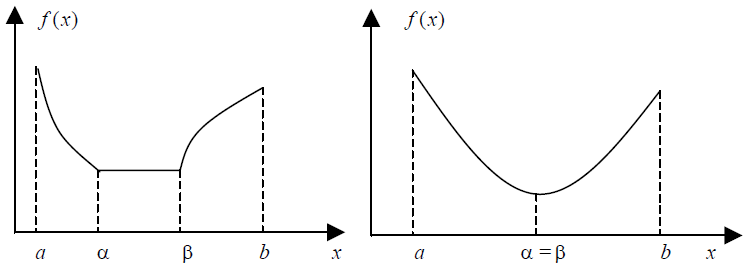
\includegraphics[width=0.8\linewidth]{unimod_example.png}}
\caption{Примеры унимодальных функций}
\label{fig:unimod_example}
\end{figure}

Прежде чем приступить к процедуре оптимизации, следует по возможности установить принадлежность целевой функции классу, для которого гарантирована сходимость процесса.

Заметим, что предположение об унимодальности функции в окрестности точки экстремума весьма естественно. Получение информации о таком промежутке является важным предварительным этапом процедуры оптимизации.

Рассмотрим с общих позиций ряд методов (разделы \ref{sec:PassiveSearch} и \ref{sec:PosledSearch}), позволяющих находить экстремумы (далее при рассмотрении алгоритмов будем говорить о задаче поиска минимума) унимодальных функций на отрезке $\left[a, b\right]$. Эти методы объединяет идея сокращения \textbf{текущего интервала неопределенности (ТИН)}. Она состоит в том, что в процессе поиска исключаются из рассмотрения те подынтервалы, на которых точка оптимума $x^{*}$ отсутствует в силу унимодальности целевой функции.

\subsection{Пассивные методы поиска}
\label{sec:PassiveSearch}
На практике подобные методы применяются, когда удобно провести независимые эксперименты по измерению значений функции $f(x)$, а последовательное измерение этих значений трудоемко или невозможно по каким-либо причинам.

\subsubsection{Метод равномерного поиска}
Испытания проводятся в точках, которые определяются путем равномерного деления отрезка $\left[a, b\right]$ на $N$ одинаковых интервалов. Из вычисленных в узлах полученной сетки значений целевой функции выбирается наименьшее (пусть это значение достигается в некотором узле $x_{k}$. Тогда, в связи с унимодальностью целевой функции, подынтервалы $\left[a, x_{k-1}\right]$ и $\left[x_{k+1}, b\right]$ можно исключить из рассмотрения, то есть сделать очередным ТИН отрезок $\left[x_{k-1}, x_{k+1}\right]$.

\textbf{Алгоритм метода:}
\begin{enumerate}
\item Выполняем присваивание $r = 1, a^{1} = a, b^{1} = b, \text{ТИН}_{1} = \left[a^{1}, b^{1}\right]$.
\item На очередном ТИН строим равномерную сетку с $N + 1$ узлом.
\item Вычисляем значения целевой функции в узлах сетки.
\item Находим минимальное из вычисленных значений $\min(f(x^{r}_{0}), f(x^{r}_{1}), \ldots, f(x^{r}_{N})) = f(x^{r}_{k})$.
\item Выполняем присваивание $a^{r+1} = x^{r}_{k-1}, b^{r+1} = x^{r}_{k+1}, \text{ТИН}_{r+1} = \left[a^{r+1}, b^{r+1}\right]$.
\item Если $\left|\text{ТИН}_{r+1}\right| \leq \epsilon_{x}$, то заканчиваем вычисления; иначе выполняем присваивание $r = r + 1$ и переходим к шагу 2.
\end{enumerate}
В качестве приближенного значения точки минимума $x^{*}$ может быть принята любая точка последнего ТИН.

На рисунке \ref{fig:uniform_search} показан один шаг метода равномерного поиска при $N = 13$.

\begin{figure}[ht]
\center{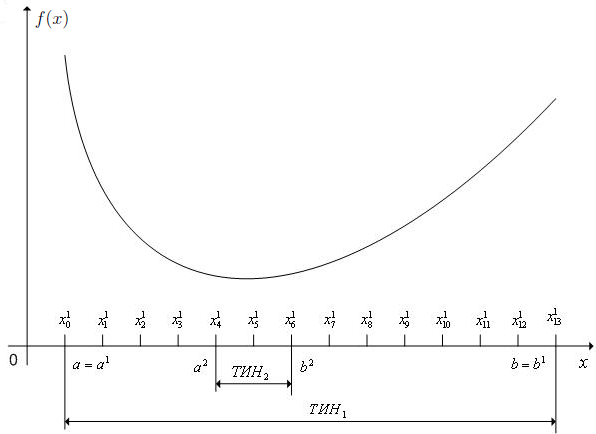
\includegraphics[width=0.8\linewidth]{uniform_search.png}}
\caption{Метод равномерного поиска}
\label{fig:uniform_search}
\end{figure}

Поскольку после каждой итерации длина ТИН уменьшается в фиксированное ($\frac{N}{2}$) количество раз, можно априорно оценить количество итераций по заданной точности решения. Действительно, после первой итерации $\left|\text{ТИН}_{2}\right| = 2\frac{b-a}{N}$, после второй итерации $\left|\text{ТИН}_{3}\right| = 2((2\frac{b-a}{N})/N) = (b-a)(\frac{2}{N})^{2}$ и т.д. Тогда после $r$-ой итерации имеем $\left|\text{ТИН}_{r+1}\right| = (b-a)(\frac{2}{N})^{r}$. Но, так как условие окончания поиска $\left|\text{ТИН}_{r+1}\right| \leq \epsilon_{x}$, получаем $(b-a)(\frac{2}{N})^{r} \leq \epsilon_{x}$. Заменив знак неравенства на равенство и выразив $r$, получим оценку количества итераций.

\subsubsection{Метод поразрядного поиска}
Можно усовершенствовать метод равномерного поиска, уменьшив количество вычислений значений целевой функции на каждой итерации. Во-первых, если $f(x^{r}_{i}) < f(x^{r}_{i+1})$, то отпадает необходимость вычислять $f(x)$ в точках $x^{r}_{i+2}, x^{r}_{i+3}$ и т.д. Во-вторых, разумно было бы сначала грубо определить отрезок, содержащий оптимальную точку; а затем на этом отрезке искать ее с меньшим шагом дискретизации. Иными словами, следует сделать шаг сетки не постоянным, а зависящим от итерации.

В методе поразрядного поиска перебор точек происходит с некоторым шагом $h_{r}$ до тех пор, пока не выполнится условие $f(x^{r}_{i}) < f(x^{r}_{i+1})$, или пока очередная из точек не совпадет с концом отрезка. После этого шаг уменьшается (обычно в 4 раза) и перебор точек с новым шагом осуществляется в противоположном направлении до тех пор, пока значения $f(x)$ снова не перестанут уменьшаться или не будет достигнут противоположный край отрезка и т.д. Описанный процесс завершается, когда перебор в каком-либо направлении закончен, а длина шага $\left|h_{r}\right| \leq \epsilon_{x}$.

\textbf{Алгоритм метода:}
\begin{enumerate}
\item Выполняем присваивание $r = 1, i = 0, x^{r}_{i} = a, h_{r} = \frac{b-a}{4}$.
\item Делаем очередной шаг $x^{r}_{i+1} = x^{r}_{i} + h_{r}$; проверяем, что $x^{r}_{i+1} \in \left[a, b\right]$: если принадлежит, то переходим к шагу 3, в противном случае - к шагу 4.
\item Вычисляем и сравниваем $f(x^{r}_{i})$ и $f(x^{r}_{i+1})$. Если $f(x^{r}_{i}) \geq f(x^{r}_{i+1})$, то положить $i = i + 1$ и перейти к шагу 2, в противном случае - к шагу 4.
\item Полагаем $x^{*} = x^{r}_{i}$ и проверяем условие окончания поиска: если $\left|h_{r}\right| \leq \epsilon_{x}$, то завершаем вычисления; в противном случае переходим к шагу 5.
\item Переходим к следующей итерации: изменяем направление поиска и уменьшаем шаг. Для этого выполняем присваивание $r = r + 1, i = 0, x^{r}_{i} = x^{*}, h_{r} = \frac{h_{r-1}}{4}$ и переходим к шагу 2.
\end{enumerate}

\subsection{Последовательные методы поиска}
\label{sec:PosledSearch}
Последовательные методы поиска на практике используются чаще, чем пассивные. Это обусловлено тем, что использование информации о результатах предыдущих измерений для выбора очередной экспериментальной точки $x_{i}$ как правило приводит к более эффективному поиску.

\subsubsection{Метод дихотомии}
В методе дихотомии испытания проводятся парами. Точки каждой последующей пары разнесены между собой на величину $\delta_{x} < \epsilon_{x}$. Испытания производятся в середине ТИН. По значениям $f(x)$, полученным в этих точках, одна половина ТИН в силу унимодальности целевой функции исключается из дальнейшего рассмотрения.

\textbf{Алгоритм метода:}
\begin{enumerate}
\item Выполняем присваивание $r = 1, a^{1} = a, b^{1} = b, \text{ТИН}_{1} = \left[a^{1}, b^{1}\right]$.
\item Вычисляем величины $x^{r}_{0} = \frac{b^{r}-a^{r}}{2}$, $x^{r}_{1} = x^{r}_{0} - \frac{\delta_{x}}{2}$, $x^{r}_{2} = x^{r}_{0} + \frac{\delta_{x}}{2}$.
\item Вычисляем значения $f(x^{r}_{1})$ и $f(x^{r}_{2})$.
\item Если $f(x^{r}_{1}) < f(x^{r}_{2})$, то выполняем присваивание $a^{r+1} = a^{r}$, $b^{r+1} = x^{r}_{0}$; в противном случае $a^{r+1} = x^{r}_{0}$, $b^{r+1} = b^{r}$. В обоих случаях $\text{ТИН}_{r+1} = \left[a^{r+1}, b^{r+1}\right]$.
\item Если $\left|\text{ТИН}_{r+1}\right| \leq \epsilon_{x}$, то заканчиваем вычисления; иначе выполняем присваивание $r = r + 1$ и переходим к шагу 2.
\end{enumerate}
В качестве приближенного значения точки минимума $x^{*}$ может быть принята любая точка последнего ТИН.

На рисунке \ref{fig:dihotom_search} показан один шаг метода дихотомии.

\begin{figure}[ht]
\center{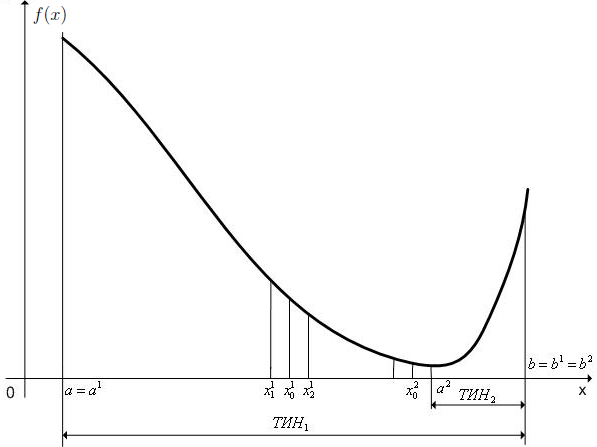
\includegraphics[width=0.8\linewidth]{dihotom_search.png}}
\caption{Метод дихотомии}
\label{fig:dihotom_search}
\end{figure}

Поскольку после каждой итерации длина ТИН уменьшается в 2 раза, можно априорно оценить количество итераций по заданной точности решения. Действительно, после первой итерации $\left|\text{ТИН}_{2}\right| = \frac{b-a}{2}$, после второй итерации $\left|\text{ТИН}_{3}\right| = ((\frac{b-a}{2})/2) = \frac{b-a}{2^{2}}$ и т.д. Тогда после $r$-ой итерации имеем $\left|\text{ТИН}_{r+1}\right| = \frac{b-a}{2^{r}}$. Но, так как условие окончания поиска $\left|\text{ТИН}_{r+1}\right| \leq \epsilon_{x}$, получаем $\frac{b-a}{2^{r}} \leq \epsilon_{x}$. Заменив знак неравенства на равенство и выразив $r$, получим оценку количества итераций.

\textit{Замечание 1}. Если производная целевой функции считается достаточно просто, можно видоизменить метод дихотомии. На концах рассматриваемого отрезка вычисляют производные целевой функции, отрезок делят пополам и вычисляют производную в средней точке. Для следующей итерации выбирают тот отрезок из двух получившихся, на концах которого знаки производной различны (по определению унимодальной функции ее производная меняет знак на отрезке поиска только один раз).

\textit{Замечание 2}. В методе дихотомии на каждой итерации значение функции вычисляется дважды. Однако, как было указано в разделе \ref{sec:ClassMetOpt}, в общем случае стараются уменьшить количество таких вычислений. Поэтому более эффективными являются методы, где новые <<экспериментальные>> точки на каждой (по возможности) итерации выбираются таким образом, чтобы значение функции приходилось вычислять только один раз.

\subsubsection{Метод Фибоначчи}
Идея метода Фибоначчи состоит в том, чтобы определять новые <<экспериментальные>> точки с помощью чисел Фибоначчи, поэтому сначала следует ввести определение и рассмотреть свойства этих чисел. Числа Фибоначчи задаются рекуррентным соотношением $F_{i} = F_{i-1} + F_{i-2}$, $i \geq 2$, $F_{0} = F_{1} = 1$. Вычислять числа Фибоначчи нерекуррентным образом можно с помощью выражения
\begin{equation}
\label{eq:num6}
F_{i} = \frac{\left(\frac{1}{\tau}\right)^{i+1}-\left(-\tau\right)^{i+1}}{\sqrt{5}},
\end{equation}
где $\tau = \frac{\sqrt{5} - 1}{2} \approx 0,618$ - решение квадратного уравнения
\begin{equation}
\label{eq:num7}
\tau^{2} + \tau - 1 = 0
\end{equation}
При больших значениях $i$ членом $\left(-\tau\right)^{i+1}$ можно пренебречь. Тогда
\begin{equation}
\label{eq:num8}
F_{i} \approx \frac{\left(\frac{1}{\tau}\right)^{i+1}}{\sqrt{5}}
\end{equation}
Можно заметить, что из \eqref{eq:num8} следует $F_{i-1} \approx \frac{\left(\frac{1}{\tau}\right)^{i}}{\sqrt{5}}$ и, следовательно,
\begin{equation}
\label{eq:num9}
\frac{F_{i-1}}{F_{i}} \approx \tau,
\end{equation}
то есть при больших $i$ отношение двух соседних чисел Фибоначчи примерно постоянно.

\textbf{Алгоритм метода} состоит из двух этапов.

Первый этап состоит из $\left(N-1\right)$-ой итерации для $r = 1, 2, \ldots, N-1$. Рассмотрим схему r-ой итерации, когда $\text{ТИН}_{r} = \left[a^{r}, b^{r}\right]$:
\begin{enumerate}
\item Вычисляем величины $x^{r}_{1} = a^{r} + \left|\text{ТИН}_{r}\right|\frac{F_{N-r-1}}{F_{N-r+1}}$, $x^{r}_{2} = a^{r} + \left|\text{ТИН}_{r}\right|\frac{F_{N-r}}{F_{N-r+1}}$.
\item Вычисляем значения $f(x^{r}_{1})$ и $f(x^{r}_{2})$.
\item Если $f(x^{r}_{1}) < f(x^{r}_{2})$, то выполняем присваивание $a^{r+1} = a^{r}$, $b^{r+1} = x^{r}_{2}$; в противном случае $a^{r+1} = x^{r}_{1}$, $b^{r+1} = b^{r}$. В обоих случаях $\text{ТИН}_{r+1} = \left[a^{r+1}, b^{r+1}\right]$.
\end{enumerate}

Данный этап алгоритма обладает тем свойством, что после выполнения $\left(N-1\right)$-ой итерации имеет место следующая ситуация: $x^{N-1}_{1} = x^{N-1}_{2} = x^{N-1}$. Таким образом, на $\left(N-1\right)$-ой итерации сужения ТИН не происходит: $\text{ТИН}_{N} = \left[a^{N-1}, b^{N-1}\right] = \text{ТИН}_{N-1}$, причем точка $x^{N-1}$ оказывается в середине $\text{ТИН}_{N-1}$.

Второй этап позволяет определить, с какой стороны от точки $x^{N-1}$ лежит точка минимума. Для этого:
\begin{enumerate}
\item Находим точку $x^{N} = x^{N-1} + \delta_{x}$, где $\delta_{x} \ll \left|\text{ТИН}_{N-1}\right|$ - свободный параметр алгоритма.
\item Вычисляем значение $f(x^{N})$.
\item Если $f(x^{N}) > f(x^{N-1})$, то выполняем присваивание $\text{ТИН}_{N+1} = \left[a^{N-1}, x^{N-1}\right]$; в противном случае $\text{ТИН}_{N+1} = \left[x^{N-1}, b^{N-1}\right]$.
\end{enumerate}
В качестве приближенного значения точки минимума $x^{*}$ может быть принята любая точка последнего ТИН.

Некоторые \textbf{свойства метода Фибоначчи}.

\textit{Утверждение 1}. Для любого $r = 1, 2, \ldots, N-2$ метод Фибоначчи обладает следующим свойством: одна из точек $x^{r+1}_{1}$, $x^{r+1}_{2}$ совпадает с одной из точек $x^{r}_{1}$, $x^{r}_{2}$.

$\blacktriangleleft$ Пусть на $r$-ой итерации выполняется $f(x^{r}_{1}) < f(x^{r}_{2})$, тогда $\text{ТИН}_{r+1} = \left[a^{r}, x^{r}_{2}\right]$ и $x^{r}_{1} \in \text{ТИН}_{r+1}$. Рассмотрим точку $x^{r+1}_{2} = a^{r} + \left|\text{ТИН}_{r+1}\right|\frac{F_{N-(r+1)}}{F_{N-(r+1)+1}} = a^{r} + \left(x^{r}_{2} - a^{r}\right)\frac{F_{N-r-1}}{F_{N-r}}$. Так как $x^{r}_{2} = a^{r} + \left|\text{ТИН}_{r}\right|\frac{F_{N-r}}{F_{N-r+1}}$, то $x^{r+1}_{2} = a^{r} + \left(a^{r} + \left|\text{ТИН}_{r}\right|\frac{F_{N-r}}{F_{N-r+1}} - a^{r}\right)\frac{F_{N-r-1}}{F_{N-r}} = a^{r} + \left|\text{ТИН}_{r}\right|\frac{F_{N-r-1}}{F_{N-r+1}} = x^{r}_{1}$ $\blacktriangleright$

Доказательство для случая $f(x^{r}_{1}) > f(x^{r}_{2})$ проводится аналогично. Указанное свойство позволяет на каждой итерации (кроме первой) производить испытания только в одной точке.

\textit{Утверждение 2}. Точки $x^{r}_{1}$, $x^{r}_{2}$ расположены симметрично относительно концов ТИН.

$\blacktriangleleft$ В соответствии с алгоритмом имеем: $x^{r}_{1} - a^{r} = a^{r} + \left(b^{r} - a^{r}\right)\frac{F_{N-r-1}}{F_{N-r+1}} - a^{r} = \left(b^{r} - a^{r}\right)\frac{F_{N-r-1}}{F_{N-r+1}}$; $b^{r} - x^{r}_{2} = b^{r} - a^{r} - \left(b^{r} - a^{r}\right)\frac{F_{N-r}}{F_{N-r+1}} = \left(b^{r} - a^{r}\right)\left(1 - \frac{F_{N-r}}{F_{N-r+1}}\right) = \left(b^{r} - a^{r}\right)\left(\frac{F_{N-r+1} - F_{N-r}}{F_{N-r+1}}\right)$. Так как из определения чисел Фибоначчи следует, что $F_{N-r} = F_{N-r+1} - F_{N-r-1}$, второе выражение можно записать как $b^{r} - x^{r}_{2} = \left(b^{r} - a^{r}\right)\frac{F_{N-r-1}}{F_{N-r+1}}$. Получили, что $x^{r}_{1} - a^{r} = b^{r} - x^{r}_{2}  \blacktriangleright$

\textit{Утверждение 3}. В результате любой итерации $r = 1, 2, \ldots, N-2$ длина ТИН уменьшается в $\frac{F_{N-r}}{F_{N-r+1}}$ раз.

$\blacktriangleleft$ Из утверждения 2 следует, что $x^{r}_{2} - a^{r} = b^{r} - x^{r}_{1}$, поэтому достаточно рассмотреть только один из отрезков $\left[a^{r}, x^{r}_{2}\right]$, $\left[x^{r}_{1}, b^{r}\right]$. Рассмотрим первый отрезок: $x^{r}_{2} - a^{r} = a^{r} + \left(b^{r} - a^{r}\right)\frac{F_{N-r}}{F_{N-r+1}} - a^{r} = \left(b^{r} - a^{r}\right)\frac{F_{N-r}}{F_{N-r+1}} \blacktriangleright$

\textit{Утверждение 4}. Из утверждения 3 и \eqref{eq:num9} следует, что при достаточно больших $N$ в результате одной итерации длина ТИН уменьшается в $\tau$ раз.

\textit{Утверждение 5}. В результате N итераций длина ТИН становится равной $\frac{b-a}{F_{N}}$.

$\blacktriangleleft$ Действительно, после первой итерации $\left|\text{ТИН}_{2}\right| = \left(b-a\right)\frac{F_{N-1}}{F_{N}}$, после второй итерации $\left|\text{ТИН}_{3}\right| = \left(b-a\right)\frac{F_{N-1}}{F_{N}}\frac{F_{N-2}}{F_{N-1}} = \left(b-a\right)\frac{F_{N-2}}{F_{N}}$ и т.д.; после $\left(N-2\right)$-ой итерации имеем $\left|\text{ТИН}_{N-1}\right| = \left(b-a\right)\frac{F_{2}}{F_{N}} = \left(b-a\right)\frac{2}{F_{N}}$, после $\left(N-1\right)$-ой итерации длина ТИН не меняется, после N-ой итерации длина ТИН уменьшается ровно в два раза (так как из утверждения 2 и выражения  $x^{N-1}_{1} = x^{N-1}_{2} = x^{N-1}$ следует, что $x^{N-1}$ делит ТИН пополам): $\left|\text{ТИН}_{N+1}\right| = \left(b-a\right)\frac{2}{F_{N}} / 2 = \frac{b-a}{F_{N}} \blacktriangleright$

Метод Фибоначчи является достаточно эффективным (см. раздел \ref{sec:EffectOneVarMethods}) методом одномерной оптимизации, однако в нем доставляет неудобство тот факт, что после выбора значения параметра $N$ следует обязательно сделать $N-1$ итераций, без возможности остановки даже в том случае, когда длина очередного ТИН стала меньше заданной точности решения. От этого недостатка можно избавиться следующим образом: из \eqref{eq:num9} следует, что отношение соседних чисел Фибоначчи примерно постоянно, следовательно, на каждой итерации можно выбирать экспериментальные точки так, чтобы они делили ТИН в одном и том же отношении $\tau$, которое не зависит от $N$. Эти рассуждения ложатся в основу метода золотого сечения.

\subsubsection{Метод золотого сечения}
Метод золотого сечения является почти таким же эффективным, как метод Фибоначчи, но позволяет остановить вычисления на любой итерации. Определение золотого сечения дается следующим образом: говорят, что точка $c$ выполняет золотое сечение отрезка $\left[a, b\right]$, если $\frac{c-a}{b-a} = \tau$.

Из определения золотого сечения следует, что $\frac{b-c}{b-a} = \frac{\left(b-a\right)-\left(c-a\right)}{b-a} = 1 -\frac{c-a}{b-a} = 1 - \tau$.

\textbf{Алгоритм метода}:
\begin{enumerate}
\item Выполняем присваивание $r = 1, a^{1} = a, b^{1} = b, \text{ТИН}_{1} = \left[a^{1}, b^{1}\right]$.
\item Вычисляем величины $x^{r}_{1} = b^{r} - \left(b^{r}-a^{r}\right)\tau$, $x^{r}_{2} = a^{r} + \left(b^{r}-a^{r}\right)\tau$.
\item Вычисляем значения $f(x^{r}_{1})$ и $f(x^{r}_{2})$.
\item Если $f(x^{r}_{1}) < f(x^{r}_{2})$, то выполняем присваивание $a^{r+1} = a^{r}$, $b^{r+1} = x^{r}_{2}$; в противном случае $a^{r+1} = x^{r}_{1}$, $b^{r+1} = b^{r}$. В обоих случаях $\text{ТИН}_{r+1} = \left[a^{r+1}, b^{r+1}\right]$.
\item Если $\left|\text{ТИН}_{r+1}\right| \leq \epsilon_{x}$, то заканчиваем вычисления; иначе выполняем присваивание $r = r + 1$ и переходим к шагу 2.
\end{enumerate}
В качестве приближенного значения точки минимума $x^{*}$ может быть принята любая точка последнего ТИН.

Некоторые \textbf{свойства метода золотого сечения}.

\textit{Утверждение 1}. Для любого $r \geq 1$ метод золотого сечения обладает следующим свойством: одна из точек $x^{r+1}_{1}$, $x^{r+1}_{2}$ совпадает с одной из точек $x^{r}_{1}$, $x^{r}_{2}$.

$\blacktriangleleft$ Пусть на $r$-ой итерации выполняется $f(x^{r}_{1}) < f(x^{r}_{2})$, тогда $\text{ТИН}_{r+1} = \left[a^{r}, x^{r}_{2}\right]$ и $x^{r}_{1} \in \text{ТИН}_{r+1}$. Чтобы доказать справедливость утверждения, нужно показать, что верно соотношение $\frac{x^{r}_{1}-a^{r}}{x^{r}_{2}-a^{r}} = \tau$. Из 2-го шага алгоритма следует, что $b^{r}-x^{r}_{1} = \left(b^{r}-a^{r}\right)\tau \Rightarrow b^{r}-x^{r}_{1}-a^{r}+a^{r} = \left(b^{r}-a^{r}\right)\tau \Rightarrow \left(b^{r}-a^{r}\right)-\left(x^{r}_{1}-a^{r}\right) = \left(b^{r}-a^{r}\right)\tau \Rightarrow x^{r}_{1} - a^{r} = \left(b^{r}-a^{r}\right)\left(1-\tau\right)$. Аналогично имеем $x^{r}_{2}-a^{r} = \left(b^{r}-a^{r}\right)\tau$. Разделив первый из полученных результатов на второй, получаем $\frac{x^{r}_{1}-a^{r}}{x^{r}_{2}-a^{r}} = \frac{1-\tau}{\tau}$. Но из \eqref{eq:num7} следует, что $1-\tau = \tau^{2}$, в результате чего имеем $\frac{x^{r}_{1}-a^{r}}{x^{r}_{2}-a^{r}} = \frac{1-\tau}{\tau} = \frac{\tau^{2}}{\tau} = \tau \blacktriangleright$

Доказательство для случая $f(x^{r}_{1}) > f(x^{r}_{2})$ проводится аналогично. Указанное свойство позволяет на каждой итерации (кроме первой) производить испытания только в одной точке.

\textit{Утверждение 2}. Точки $x^{r}_{1}$, $x^{r}_{2}$ расположены симметрично относительно концов ТИН.

$\blacktriangleleft$ Из 2-го шага алгоритма следует, что точка $x^{r}_{1}$ отстоит от точки $b^{r}$ на величину $\left(b^{r}-a^{r}\right)\tau$; точка $x^{r}_{2}$ отстоит от точки $a^{r}$ на ту же величину. $\blacktriangleright$

\textit{Утверждение 3}. Поскольку после каждой итерации длина ТИН уменьшается в $\tau$ раз, можно априорно оценить количество итераций по заданной точности решения. Действительно, после первой итерации $\left|\text{ТИН}_{2}\right| = \left(b-a\right)\tau$, после второй итерации $\left|\text{ТИН}_{3}\right| = \left(b-a\right)\tau\tau = \left(b-a\right)\tau^{2}$ и т.д. Тогда после $r$-ой итерации имеем $\left|\text{ТИН}_{r+1}\right| = \left(b-a\right)\tau^{r}$. Но, так как условие окончания поиска $\left|\text{ТИН}_{r+1}\right| \leq \epsilon_{x}$, получаем $\left(b-a\right)\tau^{r} \leq \epsilon_{x}$. Заменив знак неравенства на равенство и выразив $r$, получим оценку количества итераций.

\subsection{Сравнение эффективности методов, сокращающих ТИН}
\label{sec:EffectOneVarMethods}
Обозначим через $\Phi$ класс непрерывных унимодальных одномерных функций. Пусть множество рассматриваемых методов поиска есть $\left\{A_{1}, A_{2}, A_{3}, A_{4}\right\}$, где
\begin{itemize}
\item $A_{1}$ - метод равномерного поиска;
\item $A_{2}$ - метод дихотомии;
\item $A_{3}$ - метод Фибоначчи;
\item $A_{4}$ - метод золотого сечения.
\end{itemize}
В качестве критерия оптимальности указанных методов на классе функций $\Phi$ будем использовать максимальную длину ТИН после $m$ \textbf{испытаний}:
\begin{equation}
\label{eq:num10}
W(A) = \underset{f \in \Phi}{\max} \left|\text{ТИН}_{m}(f, A)\right|
\end{equation}
Использование подобного критерия обусловлено тем, что при решении оптимизационной задачи зачастую требуется минимизировать число испытаний (это уже обсуждалось в разделе \ref{sec:ClassMetOpt}). Но, поскольку в предыдущем разделе длина ТИН связывалась с количеством итераций (а, как было показано, почти во всех методах число итераций не совпадает с числом испытаний), необходимо в выведенных формулах сделать переход от итераций к испытаниям.

При рассмотрении метода равномерного поиска было показано, что после каждой итерации длина ТИН уменьшается в $\frac{N}{2}$ раз, а количество испытаний на каждой итерации $m = N + 1$. Следовательно, $W(A_{1}) = \frac{2}{N}\left(b-a\right) = \frac{2}{m-1}\left(b-a\right)$.

При рассмотрении метода дихотомии было показано, что после каждой итерации длина ТИН уменьшается в 2 раза, количество испытаний на каждой итерации равно 2, поэтому $m = 2N$. Следовательно, $W(A_{2}) = \frac{b-a}{2^{N}} = \frac{b-a}{2^{m/2}}$.

При рассмотрении метода Фибоначчи было показано, что в результате $N$ итераций длина ТИН становится равной $\frac{b-a}{F_{N}}$, а количество испытаний $m = N + 1$ (на первой итерации два испытания, дальше по одному испытанию на каждой итерации). Следовательно, $W(A_{3}) = \frac{b-a}{F_{m - 1}}$.

При рассмотрении метода золотого сечения было показано, что в результате $N$ итераций длина ТИН становится равной $\left(b-a\right)\tau^{N}$, а количество испытаний $m = N + 1$ (на первой итерации два испытания, дальше по одному испытанию на каждой итерации). Следовательно, $W(A_{4}) = \left(b-a\right)\tau^{m-1}$.

Пользуясь полученными результатами, сравним метод дихотомии и метод Фибоначчи при числе испытаний $m = 14$: $\frac{W(A_{2})}{W(A_{3})} = \frac{F_{m-1}}{2^{m/2}} = \frac{F_{13}}{2^{7}} = \frac{233}{128} \approx 1,82$. Видно, что метод Фибоначчи почти в два раза эффективнее метода дихотомии.

\subsection{Методы полиномиальной аппроксимации}
Если при решении оптимизационной задачи была получена информация о том, что целевая функция является достаточно гладкой в некоторой окрестности экстремума, то в этой окрестности ее можно достаточно точно заменить (аппроксимировать) полиномом некоторого порядка, после чего использовать для нахождения экстремума этот полином.

Качество аппроксимации может быть повышено двумя способами:
\begin{itemize}
\item Увеличение степени аппроксимирующего полинома;
\item Уменьшение сетки аппроксимации.
\end{itemize}
Второй способ является более предпочтительным, так как построение полинома порядка выше трех - достаточно сложная задача.

\subsubsection{Метод квадратичной аппроксимации}
В данном методе целевая функция приближенно заменяется параболой, проходящей через три известные точки $\left(x_{i}, y_{i}\right)$, где $y_{i} = f(x_{i}),\ i=1,2,3$.

Построим полином следующего вида: $q(x) = a_{0} + a_{1}(x-x_{1}) + a_{2}(x-x_{1})(x-x_{2})$. Необходимо выбрать $a_{i},\ i=1,2,3$ таким образом, чтобы $q(x_{i}) = y_{i},\ i=1,2,3$.

Подставим в полином $x_{1}$: $q(x_{1}) = a_{0}$, следовательно, $a_{0} = y_{1}$. Подставим в полином $x_{2}$: $q(x_{2}) = a_{0} + a_{1}(x_{2}-x_{1}) = y_{2}$, следовательно, $a_{1} = \frac{y_{2} - y_{1}}{x_{2} - x_{1}}$. Подставим в полином $x_{3}$: $q(x_{3}) = a_{0} + a_{1}(x_{3}-x_{1}) + a_{2}(x_{3} - x_{1})(x_{3}-x_{2}) = y_{3}$, следовательно, $a_{2} = \frac{1}{x_{3} - x_{2}}\left(\frac{y_{3}-y_{1}}{x_{3}-x_{1}} - \frac{y_{2}-y_{1}}{x_{2}-x_{1}}\right)$.

Найдем экстремум классическим методом, взяв производную: $q'(x) = a_{1} + a_{2}(x-x_{1}) + a_{2}(x-x_{2}) = 0$, откуда $x^{*} = \frac{x_{1} + x_{2}}{2} - \frac{a_{1}}{2a_{2}}$.\\

\textit{Пример}. Найдем с помощью квадратичной аппроксимации экстремум функции $f(x) = \sin(x) + \cos(x)$ на отрезке $[-1; 1]$. В качестве точек аппроксимации возьмем $x_{1} = -1,\ x_{2} = 0,\ x_{3} = 1$, и, соответственно, $y_{1} \approx -0,3,\ y_{2} = 1,\ y_{3} = 1,38$. Для определения оптимальной точки нужно знать коэффициенты $a_{1}$ и $a_{2}$. Найдем их: $a_{1} = \frac{y_{2} - y_{1}}{x_{2} - x_{1}} \approx 1,3$; $a_{2} = \frac{1}{x_{3} - x_{2}}\left(\frac{y_{3}-y_{1}}{x_{3}-x_{1}} - a_{1}\right) \approx -0,46$. Тогда $x^{*} = \frac{x_{1} + x_{2}}{2} - \frac{a_{1}}{2a_{2}} \approx 0,91$. Из рисунка \ref{fig:approx_example} видно, что построенный аппроксимационный полином достаточно точно приближает целевую функцию.

\begin{figure}[ht]
\center{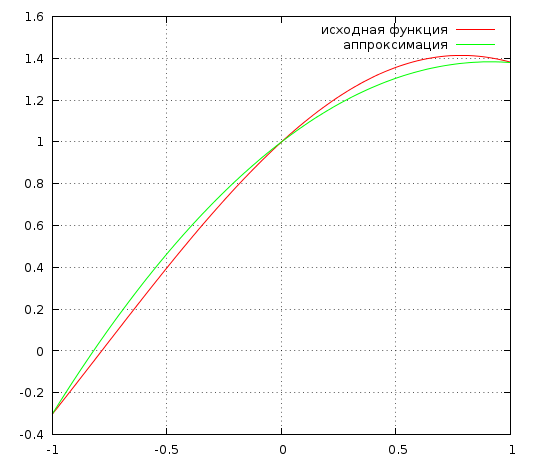
\includegraphics[width=0.8\linewidth]{approx_example.png}}
\caption{Целевая функция и аппроксимирующий полином}
\label{fig:approx_example}
\end{figure}

Подобные расчеты можно повторять для уточнения точки экстремума, на каждой итерации заново выбирая точки $x_{i},\ i=1,2,3$ каким-либо образом. Например, можно найденную на предыдущем шаге точку оптимума обозначать как $x_{2}$, а в качестве точек $x_{1}$ и $x_{3}$ брать те использовавшиеся на предыдущем шаге точки, между которыми оказалась точка оптимума. Например, для примера выше $x_{1} = -1,\ x_{2} = 0,\ x_{3} = 1$ и $x^{*} \approx 0,91$. Тогда на следующем шаге можно положить $x_{1} = 0,\ x_{2} \approx 0,91 ,\ x_{3} = 1$. Однако это не всегда возможно: скажем, вполне возможна ситуация, когда $x^{*} \notin [x_{1}; x_{3}]$; решить эту проблему помогает метод Пауэлла.

\subsubsection{Метод Пауэлла}
\begin{enumerate}
\item Выбираем начальную точку $x_{1}$, величину шага $\Delta_{x}$ и $\epsilon_{1},\ \epsilon_{2}$ - малые положительные числа.
\item Выполняем $x_{2} = x_{1} + \Delta_{x}$.
\item Вычисляем $f(x_{1})$ и $f(x_{2})$. Если $f(x_{1}) > f(x_{2})$, то $x_{3} = x_{1} + 2\Delta_{x}$; в противном случае $x_{3} = x_{1} - \Delta_{x}$.
\item Вычисляем $f(x_{3})$ и находим $f_{min} = \min\left\{f(x_{1}),f(x_{2}),f(x_{3})\right\}$; $x_{min} = \left\{x_{i} | f(x_{i}) = f_{min}\right\}$.
\item По $x_{1},\ x_{2}.\ x_{3}$ вычисляем $x^{*}$ и $f(x^{*})$, пользуясь формулами квадратичной аппроксимации. Если $a_{2}=0$, то результатом аппроксимации является не парабола, а прямая; в этом случае следует положить $x_{1}=x_{min}$ и перейти к шагу 2.
\item Проверяем условия окончания поиска: $\left|\frac{f_{min} - f(x^{*})}{f(x^{*})}\right| \leq \epsilon_{1}$, $\left|\frac{x_{min} - x^{*}}{x^{*}}\right| \leq \epsilon_{2}$.
\begin{itemize}
\item Если оба условия выполняются, останавливаем поиск; точка оптимума - $x^{*}$;
\item Если хотя бы одно условие не выполняется и $x^{*} \in [x_{1}; x_{3}]$ (или $x^{*} \in [x_{3}; x_{2}]$ - в зависимости от выбранного на шаге 3 направления поиска), то выбираем <<наилучшую точку>> (либо $x_{min}$, либо $x^{*}$) и две использовавшиеся точки по обе стороны от нее. Обозначаем эти точки в естественном порядке $x_{1},\ x_{2},\ x_{3}$ и переходим к шагу 5;
\item Если хотя бы одно условие не выполняется и $x^{*} \notin [x_{1}; x_{3}]$ (или $x^{*} \notin [x_{3}; x_{2}]$ - в зависимости от выбранного на шаге 3 направления поиска), то обозначаем $x_{1}=x_{min}$ и переходим к шагу 2.
\end{itemize}
\end{enumerate}

\subsection{Методы, использующие производные}
Если целевая функция достаточно просто дифференцируется и вычисление значения производной не представляет значительных сложностей, то целесообразно воспользоваться этим обстоятельством для поиска экстремума. Общая идея излагаемых ниже методов состоит в численном решении уравнения классического метода оптимизации - $f'(x) = 0$.

\subsubsection{Метод средней точки}
Данный метод очень схож с методом дихотомии: определяются две точки $L$ и $R$, в которых производная целевой функции имеет разные знаки (например, $f'(L) < 0,\ f'(R) > 0$). Тогда точка экстремума, в которой $f'(x) = 0$, будет находиться на отрезке $[L, R]$. Полагаем $Z = \frac{L+R}{2}$ и вычисляем $f'(Z)$, после чего исключаем из рассмотрения один из отрезков ($[L, Z]$ или $[Z, R]$), на краях которого знаки производной совпадают. Процесс можно повторять до достижения требуемой точности: $\left|R-L\right| \leq \epsilon$ или $\left|f'(Z)\right| \leq \epsilon$.

\subsubsection{Метод Ньютона (касательных)}
Если целевая функция имеет непрерывные и сохраняющие определенные знаки производные вплоть до третьей включительно на некотором отрезке $[a, b]$, причем первая производная имеет разные знаки на концах этого отрезка (то есть $f'(a)f'(b) < 0$), то, исходя из начального приближения $x_{0} \in [a, b]$, удовлетворяющего условию $f'(x_{0})f'''(x_{0}) > 0$, можно вычислить с любой точностью единственный корень уравнения $f'(x) = 0$.

Проведем через точку $(x_{0}, y_{0})$ касательную. Уравнение такой касательной записывается как
\begin{equation}
\label{eq:num11}
y = f(x_{0}) + f'(x_{0})(x-x_{0})
\end{equation}

Поскольку мы ищем решение уравнения $f'(x) = 0$, заменим в \eqref{eq:num11} $f$ на $f'$ и $f'$ на $f''$, после чего найдем точку пересечения касательной с осью абсцисс ($y = 0$): $f'(x_{0}) + f''(x_{0})(x-x_{0}) = 0$. Из полученного соотношения выразим $x$: $x = x_{0} - \frac{f'(x_{0})}{f''(x_{0})}$. Тогда можно построить итерационный процесс:
\begin{equation}
\label{eq:num12}
x_{k+1} = x_{k} - \frac{f'(x_{k})}{f''(x_{k})}
\end{equation}

Геометрическая интерпретация метода приведена на рисунке \ref{fig:newton_example}. Итерационный процесс \eqref{eq:num12} заканчивается, когда $\left|f'(x_{k+1})\right| \leq \epsilon$ или $\left|x_{k+1}-x_{k}\right| \leq \epsilon$.

\begin{figure}[ht]
\center{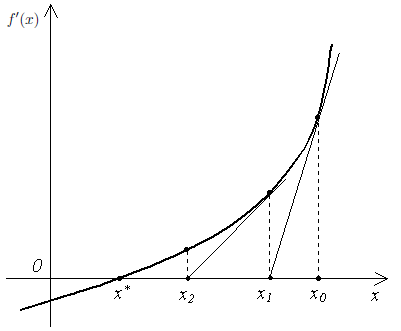
\includegraphics[width=0.8\linewidth]{newton_example.png}}
\caption{Геометрическая интерпретация метода Ньютона}
\label{fig:newton_example}
\end{figure}

\subsubsection{Метод секущих (хорд)}
Метод секущих получается из метода касательных заменой $f''(x_{k})$ в \eqref{eq:num12} разностным приближением: $f''(x_{k}) \approx \frac{f'(x_{k})-f'(x_{k-1})}{x_{k}-x_{k-1}}$. В результате получим формулу итерационного процесса:
\begin{equation}
\label{eq:num13}
x_{k+1}=x_{k}-\frac{x_{k}-x_{k-1}}{f'(x_{k})-f'(x_{k-1})}f'(x_{k})
\end{equation}

Методом хорд называют метод секущих в том случае, когда один из концов отрезка $[a, b]$ закреплен, т. е. вычисление приближения корня уравнения $f'(x) = 0$ производят по формулам:
\begin{equation}
\label{eq:num14}
x_{k+1}=x_{k}-\frac{x_{k}-a}{f'(x_{k})-f'(a)}f'(x_{k}),\ x_{0} = b
\end{equation}
либо
\begin{equation}
\label{eq:num15}
x_{k+1}=x_{k}-\frac{x_{k}-b}{f'(x_{k})-f'(b)}f'(x_{k}),\ x_{0} = a
\end{equation}

В качестве $x_{0}$ в обоих методах выбирают тот конец отрезка, на котором выполняется $f'(x_{0})f'''(x_{0}) > 0$. Для метода секущих дополнительно нужно определить $x_{1}$, так как этот метод является двухшаговым; это делается с помощью одной итерации метода хорд (см. \eqref{eq:num14}, \eqref{eq:num15}), а все последующие значения вычисляются с помощью \eqref{eq:num13}.

Геометрическая интерпретация метода хорд приведена на рисунке \ref{fig:sek_example}. Итерационный процесс \eqref{eq:num13} заканчивается, когда $\left|f'(x_{k+1})\right| \leq \epsilon$ или $\left|x_{k+1}-x_{k}\right| \leq \epsilon$.

\begin{figure}[ht]
\center{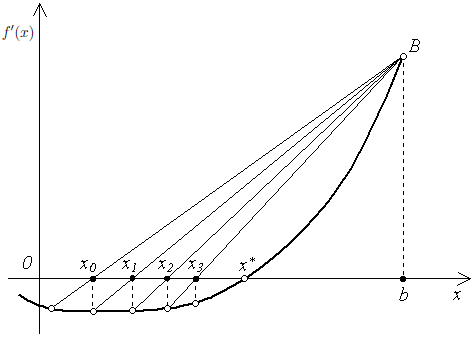
\includegraphics[width=0.8\linewidth]{sek_example.png}}
\caption{Геометрическая интерпретация метода хорд}
\label{fig:sek_example}
\end{figure}

\section{Безусловная оптимизация функций многих переменных}

\subsection{Основные понятия и определения}

\subsubsection{Постановка задачи}
Пусть задана функция $n$ действительных переменных $f(\overline{x}) = f(x_{1}, x_{2}, \ldots, x_{n})$, определенная на множестве $X \in \mathbb{R}^{n}$. Говорят, что функция $f(\overline{x})$ имеет \textbf{локальный минимум} в точке $\overline{x}^{*} \in X$, если существует окрестность точки $\overline{x}^{*}$, такая, что $f(\overline{x}^{*}) \leq f(\overline{x})$ для любой точки этой окрестности. Аналогично, функция имеет \textbf{глобальный минимум} в точке $\overline{x}^{*} \in X$, если условие $f(\overline{x}^{*}) \leq f(\overline{x})$ справедливо для любой $\overline{x} \in X$.

\subsubsection{Поверхность и линия уровня}
\textbf{Поверхностью уровня} называется геометрическое место точек, где $f(\overline{x}) = const$. Для функции двух переменных поверхность уровня называется \textbf{линией уровня}.

\subsubsection{Градиент функции многих переменных и его свойства}
Градиентом функции многих переменных называется вектор, составленный из первых частных производных функции по всем переменным:
\begin{equation}
\label{eq:num16}
\nabla f(\overline{x}) = \left(\frac{\partial f}{\partial x_{1}}, \frac{\partial f}{\partial x_{2}}, \ldots, \frac{\partial f}{\partial x_{n}}\right)^{T}
\end{equation}
Свойства градиента:
\begin{enumerate}
\item Градиент функции перпендикулярен поверхности уровня функции $f(\overline{x})$; в случае функции двух переменных он перпендикулярен касательной к линии уровня.
\item Направление градиента есть направление наиболее быстрого роста функции.
\end{enumerate}

\subsubsection{Матрица Гессе}
Квадратная матрица размера $n \times n$, состоящая из вторых частных производных функции $f(\overline{x})$, называется \textbf{матрицей Гессе}:
\begin{equation}
\label{eq:num17}
H(x) = \begin{pmatrix}
\frac{\partial^{2} f}{\partial x^{2}_{1}} & \frac{\partial^{2} f}{\partial x_{1} \partial x_{2}} & \cdots & \frac{\partial^{2} f}{\partial x_{1} \partial x_{n}} \\
\frac{\partial^{2} f}{\partial x_{2} \partial x_{1}} & \frac{\partial^{2} f}{\partial x^{2}_{2}} & \cdots & \frac{\partial^{2} f}{\partial x_{2} \partial x_{n}} \\        
\vdots & \vdots & \ddots & \vdots \\
\frac{\partial^{2} f}{\partial x_{n} \partial x_{1}} & \frac{\partial^{2} f}{\partial x_{n} \partial x_{2}} & \cdots & \frac{\partial^{2} f}{\partial x^{2}_{n}}
\end{pmatrix}
\end{equation}

\subsubsection{Критерий Сильвестра}
Матрица является \textbf{положительно определенной}, если все ее диагональные миноры положительно определены; и является \textbf{отрицательно определенной}, если все ее диагональные миноры чередуют знак, начиная со знака <<минус>>.

\subsubsection{Понятие стационарности}
Точка $\overline{x}^{*}$ называется \textbf{стационарной}, если $\nabla f(\overline{x}^{*}) = \overline{0}$ (следует понимать, что $\overline{0}$ - нулевой вектор).

\subsubsection{Условия локальной оптимальности}
\textbf{Необходимое условие} локальной оптимальности. 

Если $\overline{x}^{*}$ - точка, в которой достигается локальный экстремум, то выполняется условие стационарности $\nabla f(\overline{x}^{*}) = \overline{0}$ (обратное в общем случае неверно!).

\textbf{Достаточное условие} локальной оптимальности.

Пусть в точке $\overline{x}^{*}\ f(\overline{x})$ дважды дифференцируема и выполняется необходимое условие локальной оптимальности. Тогда, если матрица Гессе для указанной точки положительно определена, то $\overline{x}^{*}$ - точка локального минимума; если матрица Гессе для указанной точки отрицательно определена, то $\overline{x}^{*}$ - точка локального максимума; если матрица Гессе для указанной точки не определена ни положительно, ни отрицательно, то $\overline{x}^{*}$ - седловая точка.\\

\textit{Пример}. Попробуем аналитически определить точку экстремума для функции $f(x, y) = 2x^{2} + 2y^{2} + 2xy + 20x + 10y + 10$. Для этого посчитаем частные производные и составим вектор градиента: $\frac{\partial f}{\partial x} = 4x + 2y + 20,\ \frac{\partial f}{\partial y} = 4y + 2x + 10, \ \nabla f = \left(4x + 2y + 20, 4y + 2x + 10\right)^{T}$. Найдем стационарную точку из условия $\nabla f = (0, 0)^{T}$, приравняв частные производные к нулю. в результате решения системы уравнений получим $x = -5, y = 0$. Теперь построим матрицу Гессе: $H = \begin{pmatrix} \frac{\partial^{2} f}{\partial x^{2}} & \frac{\partial^{2} f}{\partial x \partial y} \\ \frac{\partial^{2} f}{\partial y \partial x} & \frac{\partial^{2} f}{\partial y^{2}} \end{pmatrix} = \begin{pmatrix} 4 & 2 \\ 2 & 4 \end{pmatrix}$. Все диагональные миноры этой матрицы положительно определены, следовательно, найденная точка является точкой минимума. График с изображением линий уровня в окрестности найденной точки это подтверждает (рис. \ref{fig:fmp_analysis_example}).

\begin{figure}[ht]
\center{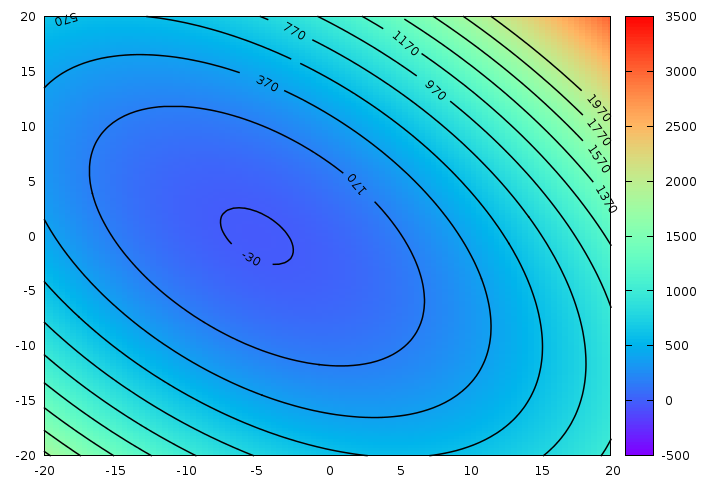
\includegraphics[width=0.8\linewidth]{fmp_analysis_example.png}}
\caption{Линии уровня в окрестности точки оптимума}
\label{fig:fmp_analysis_example}
\end{figure}

Однако, как уже было сказано, вычислять производные при решении задач оптимизации удается не всегда. Поэтому сначала рассмотрим ряд методов, позволяющих находить экстремумы функций многих переменных без вычисления частных производных.

\subsection{Простейшие поисковые методы}

\subsubsection{Метод Гаусса-Зейделя (покоординатного спуска)}
В методе Гаусса-Зейделя на каждом шаге ищут экстремум целевой функции, фиксируя все переменные, кроме какой-либо одной; значения фиксированных переменных полагаются постоянными. Поиск экстремума при одной свободной переменной выполняют любым методом одномерной оптимизации. Таким образом, в методе Гаусса-Зейделя задача многомерной оптимизации сводится к задаче одномерной оптимизации.

\textbf{Алгоритм метода:}
\begin{enumerate}
\item Выбираем начальное приближение $\overline{x}^{(0)} = (x^{(0)}_{1}, x^{(0)}_{2}, \ldots, x^{(0)}_{n})$; устанавливаем $i = 0$.
\item Фиксируем все координаты, кроме первой, и проводим операцию одномерного поиска $f(x_{1}) = f(x_{1}, x^{(i)}_{2}, x^{(i)}_{3}, \ldots, x^{(i)}_{n})$; в результате получаем $\overline{x}^{(i+1)}_{1} = (x^{*}_{1}, x^{(i)}_{2}, x^{(i)}_{3}, \ldots, x^{(i)}_{n})$.
\item Фиксируем в точке $\overline{x}^{(i+1)}_{1}$ все координаты, кроме второй, и повторяем одномерный поиск $f(x_{2}) = f(x^{*}_{1}, x_{2}, x^{(i)}_{3}, \ldots, x^{(i)}_{n})$; в результате получаем $\overline{x}^{(i+1)}_{2} = (x^{*}_{1}, x^{*}_{2}, x^{(i)}_{3}, \ldots, x^{(i)}_{n})$ и т.д. Продолжаем указанный процесс для всех $n$ координат, пока не получим $\overline{x}^{(i+1)}_{n} = (x^{*}_{1}, x^{*}_{2}, x^{*}_{3}, \ldots, x^{*}_{n})$.
\item Обозначаем $\overline{x}^{(i+1)}_{n} = \overline{x}^{(i+1)}$ и проверяем условие окончания поиска $\left\|\overline{x}^{(i+1)} - \overline{x}^{(i)}\right\| \leq \epsilon$. Если условие окончания поиска не выполняется, устанавливаем $i = i + 1$ и переходим к шагу 2; в противном случае принимаем за точку оптимума $\overline{x}^{(i+1)}$.
\end{enumerate}

Метод обладает тем недостатком, что, в случае так называемой <<овражной>> функции, оптимум никогда не будет достигнут при попадании точки в <<овраг>>.

\subsubsection{Метод Хука-Дживса (конфигураций)}
Этот метод можно рассматривать как модификацию метода Гаусса-Зейделя. Идея состоит в том, что из точки начального приближения выполняется одна итерация по методу Гаусса-Зейделя или неким аналогичным образом (<<исследующий поиск>>), а дальнейший поиск (<<поиск по образцу>>) проводят вдоль прямой, соединяющей точку начального приближения и точку, полученную во время исследующего поиска. Когда на этой прямой будет найдена точка, значение целевой функции в которой в известном смысле оптимально, из нее снова выполняют исследующий поиск и т.д.

\textbf{Алгоритм метода:}
\begin{enumerate}
\item Выбираем начальное приближение $\overline{x}^{(0)} = (x^{(0)}_{1}, x^{(0)}_{2}, \ldots, x^{(0)}_{n})$ и приращения по каждой координате $\Delta x_{j},\ j=\overline{1,n}$; устанавливаем $i = 0$.
\item \textbf{Исследующий поиск}. Рассчитываем значение целевой функции в точке $\overline{x}^{(i)}$, затем в циклическом порядке изменяем каждую координату $\overline{x}^{(i+1)}_{j} = \overline{x}^{(i)}_{j} + \Delta x_{j}$. Если такое изменение улучшает целевую функцию, то осуществляем переход к следующей координате; в противном случае делаем изменение в противоположную сторону: $\overline{x}^{(i+1)}_{j} = \overline{x}^{(i)}_{j} - \Delta x_{j}$. Если указанное действие также не привело к улучшению значения целевой функции, то значение данной координаты оставляем неизменным и переходим к следующей координате. Таким образом пробуем изменить все координаты, в результате получая точку $\overline{x}^{(i+1)}$. Если $\overline{x}^{(i+1)} = \overline{x}^{(i)}$ (то есть все попытки изменить координаты оказались <<неудачными>>), то шаг приращений следует уменьшить (обычно в два раза) и повторить исследующий поиск. Процесс вычислений следует остановить, когда размер приращений станет меньше заданной точности: $\Delta x_{j} \leq \epsilon$.
\item \textbf{Поиск по образцу}. Соединяем точки $\overline{x}^{(i+1)}$ и $\overline{x}^{(i)}$ прямой, после чего двигаемся вдоль полученного направления с некоторым шагом $k$: $\overline{x}^{(m+1)} = \overline{x}^{(m)} + k(\overline{x}^{(m)} - \overline{x}^{(m-1)})$ (на первой итерации поиска по образцу $m = i$). Данное движение выполняется до тех пор, пока в каждой новой точке $\overline{x}^{(m+1)}$ значение целевой функции улучшается. После нахождения <<оптимальной>> точки на выбранном направлении проверяем условие остановки $\Delta x_{j} \leq \epsilon$; если оно не выполнено, полагаем $i = m$ и возвращаемся к исследующему поиску (шаг 2).
\end{enumerate}

За счет возможности варьирования параметра $k$ данный метод лучше метода Гаусса-Зейделя в смысле преодоления <<оврагов>>, однако полностью исключить <<застревание в овраге>> все равно невозможно.

\subsection{Симплексные методы}
\textbf{Симплексом} в пространстве $n$ переменных называется выпуклый многогранник, имеющий $n + 1$ вершину: в пространстве 2-х переменных - это треугольник, в пространстве 3-х переменных - тетраэдр и т.д.

\subsubsection{Обычный симплекс-метод}
В обычном симплекс-методе используется правильный симплекс, все ребра которого равны. Для наглядности рассмотрим идею симплекс-метода для случая 2-х переменных.

Выбираем начальный симплекс с координатами вершин $\overline{x}^{(1)},\ \overline{x}^{(2)},\ \overline{x}^{(3)}$. Размещение этого симплекса в пространстве может быть осуществлено двумя путями.
\begin{enumerate}
\item Одна из вершин симплекса помещается в начало координат, а остальные располагаются так, чтобы ребра, выходящее из первой вершины, образовывали одинаковые углы с соответствующими координатными осями (рис. \ref{fig:simplex_1}). Координаты вершин для случая единичного симплекса приведены в таблице \ref{tab:simplex_1_2}.

\begin{minipage}{\textwidth}
  \begin{minipage}{0.49\textwidth}
    \centering
    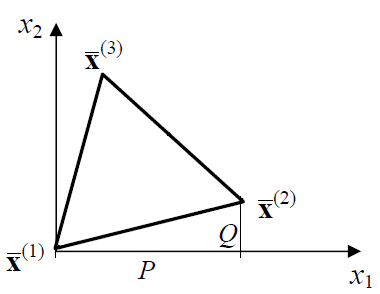
\includegraphics[width=0.7\linewidth]{simplex_1.png}
    \captionof{figure}{Симплекс с вершиной в начале координат}
    \label{fig:simplex_1}
  \end{minipage}
  \hfill
  \begin{minipage}{0.49\textwidth}
    \centering
    \captionsetup{justification=raggedleft}
    \captionof{table}{\hspace{18mm}~}
    \label{tab:simplex_1_2}
    \begin{tabular}{|c|c|c|}
      \hline
      Вершина & $x_{1}$ & $x_{2}$\\
      \hline
      $\overline{x}^{(1)}$ & 0 & 0\\
      \hline
      $\overline{x}^{(2)}$ & $\frac{\sqrt{3} + 1}{2\sqrt{2}}$ & $\frac{\sqrt{3} - 1}{2\sqrt{2}}$\\
      \hline
      $\overline{x}^{(3)}$ & $\frac{\sqrt{3} - 1}{2\sqrt{2}}$ & $\frac{\sqrt{3} + 1}{2\sqrt{2}}$\\
      \hline
    \end{tabular}
  \end{minipage}
\end{minipage}

Введя параметры $P = \frac{1}{n\sqrt{2}}(\sqrt{n+1} + n - 1)$ и $Q = \frac{1}{n\sqrt{2}}(\sqrt{n+1} - 1)$, можно расширить таблицу \ref{tab:simplex_1_2} для случая единичного симплекса в пространстве $n$ переменных (таблица \ref{tab:simplex_1_n}).

\begin{table}
\begin{center}
\captionsetup{justification=raggedleft}
\caption{\hspace{50mm}~}
\label{tab:simplex_1_n}
    \begin{tabular}{|c|c|c|c|c|c|}
      \hline
      № вершины & $x_{1}$ & $x_{2}$ & $x_{3}$ & $\ldots$ & $x_{n}$\\
      \hline
      1 & 0 & 0 & 0 & $\ldots$ & 0\\
      \hline
      2 & $P$ & $Q$ & $Q$ & $\ldots$ & $Q$\\
      \hline
      3 & $Q$ & $P$ & $Q$ & $\ldots$ & $Q$\\
      \hline
      $\ldots$ & $\ldots$ & $\ldots$ & $\ldots$ & $\ldots$ & $\ldots$\\
      \hline
      $n+1$ & $Q$ & $Q$ & $Q$ & $\ldots$ & $P$\\
      \hline
    \end{tabular}
\end{center}
\end{table}

\item Центр симплекса помещается в начало координат, а $(n+1)$-я вершина на ось $x_{n}$; остальные располагаются симметрично относительно координатных осей (рис. \ref{fig:simplex_2}). Координаты вершин для случая единичного симплекса приведены в таблице \ref{tab:simplex_2_2}.

\begin{minipage}{\textwidth}
  \begin{minipage}{0.49\textwidth}
    \centering
    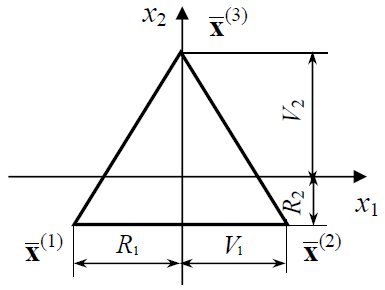
\includegraphics[width=0.7\linewidth]{simplex_2.png}
    \captionof{figure}{Симплекс с вершиной в начале координат}
    \label{fig:simplex_2}
  \end{minipage}
  \hfill
  \begin{minipage}{0.49\textwidth}
    \centering
    \captionsetup{justification=raggedleft}
    \captionof{table}{\hspace{19mm}~}
    \label{tab:simplex_2_2}
    \begin{tabular}{|c|c|c|}
      \hline
      Вершина & $x_{1}$ & $x_{2}$\\
      \hline
      $\overline{x}^{(1)}$ & $-\frac{1}{2}$ & $-\frac{1}{2\sqrt{3}}$\\
      \hline
      $\overline{x}^{(2)}$ & $\frac{1}{2}$ & $-\frac{1}{2\sqrt{3}}$\\
      \hline
      $\overline{x}^{(3)}$ & 0 & $\frac{1}{\sqrt{3}}$\\
      \hline
    \end{tabular}
  \end{minipage}
\end{minipage}

Введя параметры $R_{i} = \frac{1}{\sqrt{2i(i+1)}}$ и $V_{i} = \sqrt{\frac{i}{2(i+1)}}$, можно расширить таблицу \ref{tab:simplex_2_2} для случая единичного симплекса в пространстве $n$ переменных (таблица \ref{tab:simplex_2_n}).

\begin{table}[h]
\begin{center}
\captionsetup{justification=raggedleft}
\caption{\hspace{43mm}~}
\label{tab:simplex_2_n}
    \begin{tabular}{|c|c|c|c|c|c|}
      \hline
      № вершины & $x_{1}$ & $x_{2}$ & $x_{3}$ & $\ldots$ & $x_{n}$\\
      \hline
      1 & $-R_{1}$ & $-R_{2}$ & $-R_{3}$ & $\ldots$ & $-R_{n}$\\
      \hline
      2 & $V_{1}$ & $-R_{2}$ & $-R_{3}$ & $\ldots$ & $-R_{n}$\\
      \hline
      3 & 0 & $V_{2}$ & $-R_{3}$ & $\ldots$ & $-R_{n}$\\
      \hline
      4 & 0 & 0 & $V_{3}$ & $\ldots$ & $-R_{n}$\\
      \hline
      $\ldots$ & $\ldots$ & $\ldots$ & $\ldots$ & $\ldots$ & $\ldots$\\
      \hline
      $n+1$ & 0 & 0 & 0 & $\ldots$ & $-R_{n}$\\
      \hline
    \end{tabular}
\end{center}
\end{table}

\end{enumerate}

Как уже упоминалось, все формулы выше даны для случая единичного симплекса. Для произвольной длины ребра каждую формулу нужно дополнительно умножить на желаемую длину ребра.

Если поиск осуществляется не из начала координат, а из начальной точки $\overline{x}^{(0)}$, то к координатам вершин симплекса необходимо прибавить координаты начальной точки.

\textbf{Алгоритм метода:}
\begin{enumerate}
\item Выбираем начальное приближение $\overline{x}^{(0)}$ и строим правильный симплекс одним из предложенных способов.
\item В вершинах симплекса вычисляем значения целевой функции, выбираем из них <<худшее>> и через центр тяжести противолежащей грани строим новую вершину симплекса, симметричную <<худшей>> вершине (рис. \ref{fig:simplex_example}). Например, если <<худшая>> вершина - $\overline{x}^{(1)}$, то $\overline{x}_{\text{ц.т.}} = \frac{\overline{x}^{(2)} + \overline{x}^{(3)}}{2}$ и новая вершина $\overline{x}^{(4)} = \overline{x}_{\text{ц.т.}} + (\overline{x}_{\text{ц.т.}} - \overline{x}^{(1)}) = \overline{x}^{(2)} + \overline{x}^{(3)} - \overline{x}^{(1)}$.
\item В результате отображения <<худшей>> точки получаем новый симплекс, причем в двух его вершинах значение целевой функции уже известно. Продолжаем описанный процесс до тех пор, пока он не зациклится (отображенная вершина становится <<худшей>>). В этом случае смотрим на длину ребра симплекса - если она меньше заданной точности, то останавливаем процесс поиска; в противном случае уменьшаем размер симплекса и продолжаем поиск.
\end{enumerate}

\begin{figure}[ht]
\center{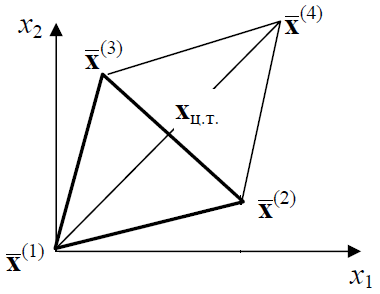
\includegraphics[width=0.5\linewidth]{simplex_example.png}}
\caption{Отображение точки с <<худшим>> значением функции}
\label{fig:simplex_example}
\end{figure}

В общем, $n$-мерном случае, если обозначить отображаемую вершину $\overline{x}^{(j)}$, то

\begin{align}
\label{eq:num18}
\begin{cases}
\overline{x}_{\text{ц.т.}} = \frac{1}{n}\sum\limits_{i \neq j}\overline{x}^{(i)} \\
\overline{x}^{(n+2)} = \overline{x}_{\text{ц.т.}} + (\overline{x}_{\text{ц.т.}} - \overline{x}^{(j)})
\end{cases}	
\end{align}

Иногда в \eqref{eq:num18} используют не зеркальное отображение, а отображение с неким коэффициентом $\alpha > 0$: $\overline{x}^{(n+2)} = \overline{x}_{\text{ц.т.}} + \alpha(\overline{x}_{\text{ц.т.}} - \overline{x}^{(j)})$, что позволяет по ходу поиска динамически менять размеры симплекса. Такая идея изменения размеров положена в основу метода Нелдера-Мида.

\subsubsection{Метод Нелдера-Мида (деформируемых многогранников)}
Данный метод является существенно более эффективным за счет того, что симплекс меняет свою форму от итерации к итерации.

\textbf{Алгоритм метода:}
\begin{enumerate}
\item Выбираем начальный (обычно правильный) симплекс с вершинами $\overline{x}^{(1)},\ \overline{x}^{(2)},\ \ldots,\ \overline{x}^{(n+1)}$ и, как в предыдущих методах, рассчитываем в этих вершинах значения целевой функции.
\item Среди вычисленных значений ищем <<наилучшее>> и <<наихудшее>> с точки зрения решаемой оптимизационной задачи. Предполагая, что мы решаем задачу на минимум, обозначим их $y_{min}$ и $y_{max}$ соответственно.
\item Отражаем <<наихудшую>> вершину относительно центра тяжести противолежащей грани с коэффициентом $\alpha$: $\overline{x}^{(n+2)} = \overline{x}_{\text{ц.т.}} + \alpha(\overline{x}_{\text{ц.т.}} - \overline{x}^{(j)})$ (обычно $\alpha = 1$), после чего вычисляем значение целевой функции в полученной точке $f(\overline{x}^{(n+2)}) = y^{(n+2)}$.
\item Анализируем результат отражения, сравнивая значения целевой функции $y^{(n+2)}$, $y_{min}$, $y_{max}$:
\begin{itemize}
\item $y^{(n+2)} < y_{min}$\\
В этом случае проводят \textbf{растяжение} симплекса, увеличивая в $\gamma > 1$ раз расстояние от отображенной вершины до центра тяжести противолежащей грани: $\overline{x}^{(n+3)} = \gamma\overline{x}^{(n+2)} + (1 - \gamma)\overline{x}_{\text{ц.т.}}$ (обычно $\gamma = 2$). Если после операции растяжения значение функции в новой точке улучшается (то есть $y^{(n+3)} \leq y^{(n+2)}$), то эта точка принимается за новую вершину очередного симплекса, в противном случае зановую вершину принимается $y^{(n+2)}$.
\item $y_{min} < y^{(n+2)} < y_{max}$\\
В этом случае проводят \textbf{сжатие} симплекса с коэффициентом $\beta < 1$: $\overline{x}^{(n+3)} = \beta\overline{x}^{(n+2)} + (1 - \beta)\overline{x}_{\text{ц.т.}}$ (обычно $\beta = 0,5$).
\item $y_{max} < y^{(n+2)}$\\
В этом случае проводят \textbf{редукцию} (уменьшение) симплекса (обычно в два раза), то есть координаты всех вершин симплекса сдвигаются на половину расстояния до наилучшей точки: $\overline{x}^{(i)} = \overline{x}_{min} + 0,5(\overline{x}^{(i)} - \overline{x}_{min}),\ i=\overline{1,n+1}$.
\end{itemize}
\end{enumerate}

В качестве критерия останова авторы метода рекомендуют среднеквадратичную величину разности значений функции в вершинах симплекса и среднего ее значения:\\ $\sqrt{\frac{1}{n+1}\sum\limits_{i=1}^{n+1}\left[f(\overline{x}^{(i)}) - f(\overline{x}_{\text{ц.т.}})\right]^{2}} \leq \epsilon$

\subsection{Градиентные методы}
Суть всех градиентных методов заключается в использовании вектора градиента для определения направления движения к экстремуму. Свойства градиента, обуславливающие его эффективное применение при поиске, уже приводились ранее:
\begin{itemize}
\item Поиск в направлении вектора градиента (антиградиента) дает быструю сходимость, так как градиент (антиградиент) всегда направлен в сторону наиболее быстрого роста (убывания) функции.
\item Условие стационарности (в точке экстремума градиент обращается в ноль) используется для проверки условия окончания поиска, то есть $\left\|\nabla f(\overline{x})\right\| \leq \epsilon$.
\end{itemize}
 
Общий алгоритм всех градиентных методов заключается в построении из некоторой начальной точки $\overline{x}^{(0)}$ последовательности приближений

\begin{equation}
\label{eq:num19}
\overline{x}^{(k+1)} = \overline{x}^{(k)} - \lambda^{(k)}\overline{s}^{(k)}\text{, где}
\end{equation}

\begin{itemize}
\item Знак <<$-$>> в правой части говорит о том, что ищется минимум целевой функции (направление антиградиента); при поиске максимума следует использовать знак <<$+$>>.
\item $\lambda^{(k)}$ - величина шага.
\item $\overline{s}^{(k)}$ - единичный вектор в направлении градиента целевой функции в точке $\overline{x}^{(k)}$: $\overline{s}^{(k)} = \frac{\nabla f(\overline{x}^{(k)})}{\left\|\nabla f(\overline{x}^{(k)})\right\|} = \frac{\nabla f(\overline{x}^{(k)})}{\sqrt{\left(\frac{\partial f}{\partial x_{1}}\right)^{2} + \left(\frac{\partial f}{\partial x_{2}}\right)^{2} + \cdots + \left(\frac{\partial f}{\partial x_{n}}\right)^{2}}}$
\end{itemize}

Следует заметить, что применение градиентных методов не всегда возможно, так как посчитать частные производные целевой функции не всегда просто (а иногда и невозможно). Поэтому в данном разделе кратко рассмотрим два метода, базирующихся на итерационном процессе \eqref{eq:num19}: простой градиентный метод и метод наискорейшего спуска; а также метод Бокса-Уилсона, позволяющий выполнить оценку значения градиента без его непосредственного вычисления.

\subsubsection{Простой градиентный метод}
Суть простого градиентного метода заключается в использовании итерационного процесса \eqref{eq:num19} с фиксированным значением шага: $\lambda^{(k)} = \lambda = const$, $\overline{x}^{(k+1)} = \overline{x}^{(k)} - \lambda\overline{s}^{(k)}$.

\subsubsection{Метод наискорейшего спуска}
В методе наискорейшего спуска шаг варьируется на каждой итерации и определяется решением одномерной задачи оптимизации: $\lambda^{(k)} = \underset{\lambda}{argmin}f(\overline{x}^{(k)} - \lambda\overline{s}^{(k)})$.

\subsubsection{Метод Бокса-Уилсона (крутого восхождения)}
Этот метод представляет собой пошаговую процедуру движения по поверхности целевой функции, в которой для оценки составляющих градиента $\nabla f(\overline{x}^{(k)}) = \left(b^{(k)}_{1}, \ldots, b^{(k)}_{n}\right)^{T}$ используется линейное уравнение регрессии $r(\overline{x}) = b^{(k)}_{0} + b^{(k)}_{1}x_{1} + \ldots + b^{(k)}_{n}x_{n}$, полученное в результате планирования эксперимента в окрестности точки $\overline{x}^{(k)}$.

Затем совершается движение по поверхности целевой функции в направлении градиента (антиградиента) с величиной шага, пропорциональной  произведению коэффициента $b^{(k)}_{j}$ на интервал варьирования $\Delta x_{j}$. Движение осуществляется до тех пор, пока значение целевой функции не начнет уменьшаться (увеличиваться). В полученной точке вновь производится планирование эксперимента и оценка нового направления движения.

Рассмотрим для наглядности случай функции двух переменных. Пусть мы имеем функцию $f(x_{1}, x_{2})$. Выбираем начальную точку поиска $\overline{x}^{(0)} = (x^{(0)}_{1}, x^{(0)}_{2})^{T}$. В окрестности этой точки проводим полный факторный эксперимент (ПФЭ) размерности $N = k^{n}$, где $k$ - количество уровней варьирования, $n$ - количество факторов; в нашем случае $N = 2^{2} = 4$. Графическая интерпретация этого процесса приведена на рисунке \ref{fig:plan_exp}. По сути дела, в данном случае ПФЭ помогает выбрать экспериментальные точки, в которых будут рассчитаны значения функции. Для удобства эти расчеты можно записать в виде матрицы планирования эксперимента (таблица \ref{tab:plan_matrix_code}).

\begin{minipage}{\textwidth}
  \begin{minipage}{0.49\textwidth}
    \centering
    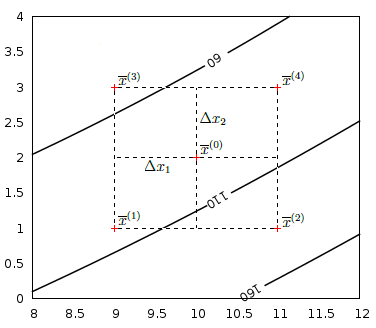
\includegraphics[width=0.9\linewidth]{plan_exp.png}
    \captionof{figure}{ПФЭ в окрестности начальной точки}
    \label{fig:plan_exp}
  \end{minipage}
  \hfill
  \begin{minipage}{0.49\textwidth}
    \centering
    \captionsetup{justification=raggedleft}
    \captionof{table}{\hspace{12mm}~}
    \label{tab:plan_matrix_code}
    \begin{tabular}{|c|c|c|c|}
      \hline
      Вершина & $X_{1}$ & $X_{2}$ & $y = f(\overline{x})$\\
      \hline
      $\overline{x}^{(1)}$ & $-1$ & $-1$ & $y_{1}$\\
      \hline
      $\overline{x}^{(2)}$ & $1$ & $-1$ & $y_{2}$\\
      \hline
      $\overline{x}^{(3)}$ & $-1$ & $1$ & $y_{3}$\\
      \hline
      $\overline{x}^{(4)}$ & $1$ & $1$ & $y_{4}$\\
      \hline
    \end{tabular}
  \end{minipage}
\end{minipage}
\\

Матрица планирования \ref{tab:plan_matrix_code} представлена в кодированных переменных. Переход от кодированных к натуральным переменным осуществляется по формуле $x_{j} = x^{(0)}_{j} + X_{j}\Delta x_{j}$, $j=\overline{1,n}$. Здесь $x^{(0)}_{j}$ - $j$-ая координата начальной точки, $X_{j}$ - кодированное значение переменной ($-1$ или $+1$), $\Delta x_{j}$ - интервал варьирования. Тогда матрица планирования в натуральных переменных будет иметь вид, представленный в таблице \ref{tab:plan_matrix_nat}:

\begin{center}
  \captionsetup{justification=raggedleft}
  \captionof{table}{\hspace{48mm}~}
  \label{tab:plan_matrix_nat}
  \begin{tabular}{|c|c|c|c|}
    \hline
    Вершина & $x_{1}$ & $x_{2}$ & $y$\\
    \hline
    $\overline{x}^{(1)}$ & $x^{(0)}_{1}-\Delta x_{1}$ & $x^{(0)}_{2}-\Delta x_{2}$ & $y_{1}$\\
    \hline
    $\overline{x}^{(2)}$ & $x^{(0)}_{1}+\Delta x_{1}$ & $x^{(0)}_{2}-\Delta x_{2}$ & $y_{2}$\\
    \hline
    $\overline{x}^{(3)}$ & $x^{(0)}_{1}-\Delta x_{1}$ & $x^{(0)}_{2}+\Delta x_{2}$ & $y_{3}$\\
    \hline
    $\overline{x}^{(4)}$ & $x^{(0)}_{1}+\Delta x_{1}$ & $x^{(0)}_{2}+\Delta x_{2}$ & $y_{4}$\\
    \hline
  \end{tabular}
\end{center}

Положив для простоты $\Delta x_{1} = \Delta x_{2} = 1$, получим матрицу \ref{tab:plan_matrix_end}:

\begin{center}
  \captionsetup{justification=raggedleft}
  \captionof{table}{\hspace{54mm}~}
  \label{tab:plan_matrix_end}
  \begin{tabular}{|c|c|c|c|}
    \hline
    Вершина & $x_{1}$ & $x_{2}$ & $y$\\
    \hline
    $\overline{x}^{(1)}$ & $x^{(0)}_{1}-1$ & $x^{(0)}_{2}-1$ & $y_{1}$\\
    \hline
    $\overline{x}^{(2)}$ & $x^{(0)}_{1}+1$ & $x^{(0)}_{2}-1$ & $y_{2}$\\
    \hline
    $\overline{x}^{(3)}$ & $x^{(0)}_{1}-1$ & $x^{(0)}_{2}+1$ & $y_{3}$\\
    \hline
    $\overline{x}^{(4)}$ & $x^{(0)}_{1}+1$ & $x^{(0)}_{2}+1$ & $y_{4}$\\
    \hline
  \end{tabular}
\end{center}

Метод ПФЭ позволяет получить коэффициенты $b_{i}$ для уравнения регрессии $r(\overline{x}) = b_{0} + b_{1}x_{1} + \ldots + b_{n}x_{n}$ по формуле $b_{i} = \frac{1}{N}\sum\limits_{j=1}^N X_{ij}y_{j}$, $i=\overline{1,n}$, $j=\overline{1,N}$. Тогда в рассматриваемом двумерном случае имеем $b_{1} = \frac{1}{4}\left(-y_{1}+y_{2}-y_{3}+y_{4}\right)$, $b_{2} = \frac{1}{4}\left(-y_{1}-y_{2}+y_{3}+y_{4}\right)$.

Коэффициенты $b_{i}$ дают оценку градиента, которую можно использовать для выбора направления движения. При таком подходе при поиске минимума координаты новых точек вычисляются по формуле $x^{(k)}_{j} = x^{(0)}_{j} - kab_{j}\Delta x_{j}$ (при поиске максимума знак <<->> в формуле меняется на <<+>>). Здесь $x^{(k)}_{j}$ - значение $j$-ой координаты на $k$-ом шаге, $a$ - коэффициент пропорциональности (выбирается с учетом вида функции).

Движение осуществляется до тех пор, пока значение функции не будет увеличиваться (уменьшаться). В точке, где был достигнут минимум (максимум) вновь реализуется ПФЭ, рассчитываются коэффициенты регресии и осуществляется движение в новом направлении и т.д. Поиск заканчивается, когда $\left\|\nabla f(\overline{x})\right\| = \sqrt{b^{2}_{1} + \ldots + b^{2}_{n}} \leq \epsilon$.

\subsection{Пример использования}
В заключение данного раздела рассмотрим использование методов многомерной безусловной оптимизации на примере самого интересного, пожалуй, метода - Бокса-Уилсона. Определим минимум функции $f(x_{1}, x_{2}) = \left(x_{1} - x_{2}\right)^{2} + \left(x_{2} - 7\right)^{2}$ с точностью $\epsilon = 0,25$, используя в качестве начальной точки $\overline{x}^{(0)} = (10;\ 2)^{T}$.

Для начала выберем интервалы варьирования, для простоты расчетов положив $\Delta x_{1} = \Delta x_{2} = 1$. Теперь можно реализовать ПФЭ размерности $N = 2^{2} = 4$, используя в качестве основной точки $x^{(0)}$. Матрица планирования \ref{tab:example_bw_1} будет иметь вид (вместе с натуральными значениями переменных в скобках записаны кодированные):

\begin{center}
  \captionsetup{justification=raggedleft}
  \captionof{table}{\hspace{54mm}~}
  \label{tab:example_bw_1}
  \begin{tabular}{|c|c|c|c|}
    \hline
    Вершина & $x_{1}$ & $x_{2}$ & $y$\\
    \hline
    $\overline{x}^{(1)}$ & 9 (-1) & 1 (-1) & 100\\
    \hline
    $\overline{x}^{(2)}$ & 11 (+1) & 1 (-1) & 136\\
    \hline
    $\overline{x}^{(3)}$ & 9 (-1) & 3 (+1) & 52\\
    \hline
    $\overline{x}^{(4)}$ & 11 (+1) & 3 (+1) & 80\\
    \hline
  \end{tabular}
\end{center}

Рассчитаем коэффициенты $b_{i}$, дающие оценку градиента: 

\begin{equation*}
b_{1} = \frac{1}{4}\left(-100+136-52+80\right) = 16
\end{equation*}

\begin{equation*}
b_{2} = \frac{1}{4}\left(-100-136+52+80\right) = -26
\end{equation*}

Проверим выполнение условия останова: $\left\|\nabla f(\overline{x})\right\| = \sqrt{b^{2}_{1} + b^{2}_{2}} \approx 30,53 > \epsilon$, то есть условие не выполняется.

Рассчитаем величину шагов по каждой координате, положив коэффициент пропорциональности $a = 0,1$: 

\begin{equation*}
h_{1} = ab_{1}\Delta x_{1} = 0,1\cdot16\cdot1 = 1,6
\end{equation*}

\begin{equation*}
h_{2} = ab_{2}\Delta x_{2} = 0,1\cdot(-26)\cdot1 = -2,6
\end{equation*}

Теперь можно начать двигаться в направлении антиградиента, используя формулы: 

\begin{equation*}
x^{(k)}_{1} = x^{(0)}_{1} - kh_{1} = 10 - 1,6k
\end{equation*}

\begin{equation*}
x^{(k)}_{2} = x^{(0)}_{2} - kh_{2} = 2+2,6k
\end{equation*}

Данные шаги показаны в таблице \ref{tab:example_bw_2}:

\begin{center}
  \captionsetup{justification=raggedleft}
  \captionof{table}{\hspace{64mm}~}
  \label{tab:example_bw_2}
  \begin{tabular}{|c|c|c|c|}
    \hline
    Шаг & $x_{1}$ & $x_{2}$ & $y$\\
    \hline
    0 & 10 & 2 & 89\\
    \hline
    1 & 8,4 & 4,6 & 20,2\\
    \hline
    2 & 6,8 & 7,2 & 0,2\\
    \hline
    3 & 5,2 & 9,8 & 29\\
    \hline
  \end{tabular}
\end{center}

Из таблицы \ref{tab:example_bw_2} видно, что функция перестала убывать после 2-го шага. Таким образом, новой начальной точкой становится $\overline{x}^{(2)} = (6,8;\ 7,2)^{T}$.

Реализуем ПФЭ размерности $N = 2^{2} = 4$. Матрица планирования \ref{tab:example_bw_3} будет иметь вид:

\begin{center}
  \captionsetup{justification=raggedleft}
  \captionof{table}{\hspace{52mm}~}
  \label{tab:example_bw_3}
  \begin{tabular}{|c|c|c|c|}
    \hline
    Вершина & $x_{1}$ & $x_{2}$ & $y$\\
    \hline
    $\overline{x}^{(1)}$ & 5,8 (-1) & 6,2 (-1) & 0,8\\
    \hline
    $\overline{x}^{(2)}$ & 7,8 (+1) & 6,2 (-1) & 3,2\\
    \hline
    $\overline{x}^{(3)}$ & 5,8 (-1) & 8,2 (+1) & 7,2\\
    \hline
    $\overline{x}^{(4)}$ & 7,8 (+1) & 8,2 (+1) & 1,6\\
    \hline
  \end{tabular}
\end{center}

Рассчитаем коэффициенты $b_{i}$, дающие оценку градиента: 

\begin{equation*}
b_{1} = \frac{1}{4}\left(-0,8+3,2-7,2+1,6\right) = -0,8
\end{equation*}

\begin{equation*}
b_{2} = \frac{1}{4}\left(-0,8-3,2+7,2+1,6\right) = 1,2
\end{equation*}

Проверим выполнение условия останова: $\left\|\nabla f(\overline{x})\right\| = \sqrt{b^{2}_{1} + b^{2}_{2}} \approx 1,44 > \epsilon$, то есть условие не выполняется.

Рассчитаем величину шагов по каждой координате:

\begin{equation*}
h_{1} = ab_{1}\Delta x_{1} = 0,1\cdot(-0,8)\cdot1 = -0,08
\end{equation*}

\begin{equation*}
h_{2} = ab_{2}\Delta x_{2} = 0,1\cdot1,2\cdot1 = 0,12
\end{equation*}

Теперь можно начать двигаться в направлении антиградиента, используя формулы:

\begin{equation*}
x^{(k)}_{1} = 6,8 + 0,08k
\end{equation*}

\begin{equation*}
x^{(k)}_{2} = 7,2 - 0,12k
\end{equation*}

Данные шаги показаны в таблице \ref{tab:example_bw_4}:

\begin{center}
  \captionsetup{justification=raggedleft}
  \captionof{table}{\hspace{59mm}~}
  \label{tab:example_bw_4}
  \begin{tabular}{|c|c|c|c|}
    \hline
    Шаг & $x_{1}$ & $x_{2}$ & $y$\\
    \hline
    0 & 6,8 & 7,2 & 0,2\\
    \hline
    1 & 6,88 & 7,08 & 0,0464\\
    \hline
    2 & 6,96 & 6,96 & 0,0016\\
    \hline
    3 & 7,04 & 6,84 & 0,0656\\
    \hline
  \end{tabular}
\end{center}

Из таблицы \ref{tab:example_bw_4} видно, что функция перестала убывать после 2-го шага. Таким образом, новой начальной точкой становится $\overline{x}^{(2)} = (6,96;\ 6,96)^{T}$.

Реализуем ПФЭ размерности $N = 2^{2} = 4$. Матрица планирования \ref{tab:example_bw_5} будет иметь вид:

\begin{center}
  \captionsetup{justification=raggedleft}
  \captionof{table}{\hspace{46mm}~}
  \label{tab:example_bw_5}
  \begin{tabular}{|c|c|c|c|}
    \hline
    Вершина & $x_{1}$ & $x_{2}$ & $y$\\
    \hline
    $\overline{x}^{(1)}$ & 5,96 (-1) & 5,96 (-1) & 1,0816\\
    \hline
    $\overline{x}^{(2)}$ & 7,96 (+1) & 5,96 (-1) & 5,0816\\
    \hline
    $\overline{x}^{(3)}$ & 5,96 (-1) & 7,96 (+1) & 4,9216\\
    \hline
    $\overline{x}^{(4)}$ & 7,96 (+1) & 7,96 (+1) & 0,9216\\
    \hline
  \end{tabular}
\end{center}

Рассчитаем коэффициенты $b_{i}$, дающие оценку градиента:

\begin{equation*}
b_{1} = \frac{1}{4}\left(-1,0816 + 5,0816 - 4,9216 + 0,9216\right) = 0
\end{equation*}

\begin{equation*}
b_{2} = \frac{1}{4}\left(-1,0816 - 5,0816 + 4,9216 + 0,9216\right) = -0,08
\end{equation*}

Проверим выполнение условия останова: $\left\|\nabla f(\overline{x})\right\| = \sqrt{b^{2}_{1} + b^{2}_{2}} = 0,08 < \epsilon$, то есть условие выполняется и поиск нужно остановить. Таким образом, точка $\overline{x} = (6,96;\ 6,96)^{T}$ есть точка оптимума.

Траектория поиска изображена на рисунке \ref{fig:example_bw_graph}.

\newpage

\begin{figure}[ht]
\center{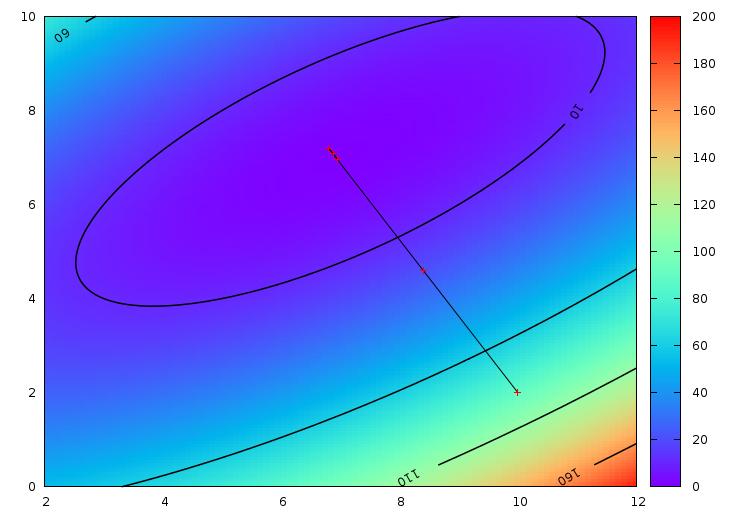
\includegraphics[width=1\linewidth]{example_bw_graph.png}}
\caption{Траектория поиска по методу Бокса-Уилсона}
\label{fig:example_bw_graph}
\end{figure}

Следует отметить достаточно высокую скорость приближения к оптимальной точке, что обусловлено использованием оценки градиента для выбора направления поиска. На рисунке хорошо видно, что траектория поиска фактически является перпендикуляром к касательным линий уровня.

\clearpage

\chapter{Линейное программирование}

\section{Постановка задачи и основные определения}

\textbf{Общей задачей} линейного программирования называется задача, которая состоит в определении \textit{максимального} (минимального) значения функции

\begin{equation}
\label{eq:num20}
F = \sum\limits_{j=1}^n c_{j}x_{j}
\end{equation}
при ограничениях
\begin{equation}
\label{eq:num21}
\sum\limits_{j=1}^n a_{ij}x_{j} \leq b_{i},\ i=\overline{1,k}
\end{equation}
\begin{equation}
\label{eq:num22}
\sum\limits_{j=1}^n a_{ij}x_{j} = b_{i},\ i=\overline{k+1,m}
\end{equation}
\begin{equation}
\label{eq:num23}
x_{j} \geq 0, j=\overline{1,l},\ l \leq n
\end{equation}

Целевая функция \eqref{eq:num20} называется \textbf{линейной формой} задачи \eqref{eq:num20}-\eqref{eq:num23}, условия \eqref{eq:num21}-\eqref{eq:num23} называются \textbf{ограничениями} данной задачи.

\textbf{Канонической (основной) задачей} линейного программирования (далее - \textbf{ОЗЛП}) называется задача, которая состоит в определении максимального значения функции \eqref{eq:num20} при ограничениях \eqref{eq:num22}-\eqref{eq:num23}, где $k = 0$ и $l = n$.

Совокупность чисел $(x_{1}, \ldots, x_{n}) = X$, удовлетворяющих ограничениям \eqref{eq:num21}-\eqref{eq:num23}, называется \textbf{допустимым решением} или \textbf{планом}.

План $X^{*}$, при котором функция \eqref{eq:num20} принимает максимальное (минимальное) значение, называется \textbf{оптимальным}.

\section{Переход от общей к основной задаче линейного программирования}

Чтобы перейти от общей к основной задаче линейного программирования, нужно в общем случае уметь:

\begin{enumerate}
\item Переходить от задачи минимизации к задаче максимизации. 

Это делается заменой знака в линейной форме:
\begin{equation*}
\min F = c_{1}x_{1} + c_{2}x_{2} + \ldots + c_{n}x_{n} \Leftrightarrow \max (-F) = -c_{1}x_{1} - c_{2}x_{2} - \ldots - c_{n}x_{n}
\end{equation*}

\item Переходить от ограничений-неравенств к ограничениям-равенствам. 

Неравенство вида <<$\leq$>> можно преобразовать в равенство добавлением к его левой части дополнительной неотрицательной переменной:
\begin{equation*}
a_{i1}x_{1} + a_{i2}x_{2} + \ldots + a_{in}x_{n} \leq b_{i} \Leftrightarrow a_{i1}x_{1} + a_{i2}x_{2} + \ldots + a_{in}x_{n} + x_{n+1} = b_{i},\ x_{n+1} \geq 0
\end{equation*}

Неравенство вида <<$\geq$>> можно преобразовать в равенство вычитанием из его левой части дополнительной неотрицательной переменной:
\begin{equation*}
a_{i1}x_{1} + a_{i2}x_{2} + \ldots + a_{in}x_{n} \geq b_{i} \Leftrightarrow a_{i1}x_{1} + a_{i2}x_{2} + \ldots + a_{in}x_{n} - x_{n+1} = b_{i},\ x_{n+1} \geq 0
\end{equation*}

\item Делать замену переменных, которые не подчинены условию неотрицательности.

Если некоторая переменная $x_{j}$ не подчинена условию неотрицательности, то ее заменяют двумя неотрицательными переменными $u_{j} \geq 0$ и $v_{j} \geq 0$ (они берутся произвольно): $x_{j} = u_{j} - v_{j}$.
\end{enumerate}

\section{Существование допустимых решений ОЗЛП}
ОЗЛП необязательно должна иметь решение. Может оказаться, что ограничения задачи противоречат друг другу; может оказаться, что решение есть, но не в области отрицательных значений переменных и т.д. Как же узнать, существует или не существует допустимое решение (или решения) ОЗЛП?

Заметим, что ограничения ОЗЛП суть система линейных алгебраических уравнений (СЛАУ):

\begin{align*}
\begin{cases}
a_{11}x_{1} + a_{12}x_{2} + \ldots + a_{1n}x_{n} = b_{1} \\
a_{21}x_{1} + a_{22}x_{2} + \ldots + a_{2n}x_{n} = b_{2} \\
\ldots \\
a_{m1}x_{1} + a_{m2}x_{2} + \ldots + a_{mn}x_{n} = b_{m} \\
\end{cases}	
\Longleftrightarrow Ax = b,
\end{align*}

\begin{equation*}
A = \begin{pmatrix}
a_{11} & a_{12} & \cdots & a_{1n} \\
a_{21} & a_{22} & \cdots & a_{2n} \\        
\vdots & \vdots & \ddots & \vdots \\
a_{m1} & a_{m2} & \cdots & a_{mn}
\end{pmatrix},\ x = \begin{pmatrix}
x_{1} \\
x_{2} \\        
\vdots \\
x_{n}
\end{pmatrix},\ b = \begin{pmatrix}
b_{1} \\
b_{2} \\        
\vdots \\
b_{m}
\end{pmatrix}
\end{equation*}

Из курса линейной алгебры известно, что для совместности СЛАУ необходимо и достаточно, чтобы ранг ее матрицы был равен рангу ее расширенной матрицы (рангом матрицы называется наибольший порядок отличного от нуля определителя, который можно получить, вычеркивая из матрицы какие-либо строки и какие-либо столбцы).

Тогда, если система ограничений ОЗЛП совместна, то матрица системы и ее расширенная матрица имеют один и тот же ранг; обозначим его $r$. Таким образом, $r$ - число линейно-независимых уравнений среди ограничений ОЗЛП.

Очевидно, что ранг системы не может быть больше числа уравнений системы, то есть $r \leq m$. Очевидно, что ранг системы не может быть больше числа переменных задачи, то есть $r \leq n$.

Рассмотрим случай, когда $r = n$. Отбросим линейно-зависимые уравнения-ограничения и получим систему:

\begin{align*}
\begin{cases}
a_{11}x_{1} + a_{12}x_{2} + \ldots + a_{1n}x_{n} = b_{1} \\
a_{21}x_{1} + a_{22}x_{2} + \ldots + a_{2n}x_{n} = b_{2} \\
\ldots \\
a_{n1}x_{1} + a_{n2}x_{2} + \ldots + a_{nn}x_{n} = b_{n} \\
\end{cases}	
\end{align*}

Так как $r = n$, то определитель матрицы этой системы не равен нулю. Из курса линейной алгебры известно, что в этом случае система имеет единственное решение. Если в этом решении хотя бы одна из переменных $x_{i}, i=\overline{1,n}$ отрицательна, то решение недопустимо и, следовательно, ОЗЛП не имеет решения. Если же все переменные положительны, то найденное решение является допустимым и оптимальным (так как других решений нет).

Очевидно, что такой тривиальный случай малоинтересен, поэтому в дальнейшем будем рассматривать случаи, когда $r < n$, то есть число линейно-независимых ограничений меньше числа переменных в задаче. Тогда, если система ограничений совместна, у нее существует бесчисленное множество решений. При этом $n-r$ переменным можно придавать произвольные значения (будем называть их \textbf{свободными} переменными), а остальные $r$ переменных выразятся через них (будем называть эти переменные \textbf{базисными}).

В дальнейшем, для простоты, будем полагать все ограничения ОЗЛП линейно-независимыми, то есть $r = m$. Тогда, если $m < n$, система ограничений имеет бесконечно множество решений. Если среди этих решений нет ни одного, для которого все $x_{i}, i=\overline{1,n}$ неотрицательны, то ОЗЛП не имеет допустимого решения. Если же существуют решения, для которых все переменные положительны, то каждое из них допустимо. Возникает задача отыскания среди них оптимального решения.

Для того, чтобы лучше представить себе ход решения ОЗЛП и различные случаи, которые могут при этом встретиться, удобно воспользоваться геометрической интерпретацией.

\section{Геометрическая интерпретация ОЗЛП}
\label{sec:LP_Geom}
Рассмотрим случай, когда число переменных на два больше, чем число линейно-независимых ограничений, то есть $n - m = 2$. Тогда можно две переменные выбрать в качестве свободных (пусть это будут $x_{1}$ и $x_{2}$), а остальные $m = n - 2$ сделать базисными и выразить через свободные.

Получим $m = n - 2$ уравнений вида:

\begin{align*}
\begin{cases}
x_{3} = \alpha_{31}x_{1} + \alpha_{32}x_{2} + \beta_{3} \geq 0 \\
x_{4} = \alpha_{41}x_{1} + \alpha_{42}x_{2} + \beta_{4} \geq 0 \\
\ldots \\
x_{n} = \alpha_{n1}x_{1} + \alpha_{n2}x_{2} + \beta_{n} \geq 0 \\
\end{cases}	
\end{align*}

Изобразим на рисунке прямые $x_{i} = 0, i=\overline{1,n}$ (рис. \ref{fig:linogr_geom}). Свободные переменные в этом случае образуют <<координатные оси>>, а базисные переменные - некоторые прямые в количестве $n-2$ штук. Так как на все переменные наложено условие неотрицательности, допустимые значения свободных переменных лежат в первой четверти <<координатной>> плоскости, а допустимые значения базисных переменных - по ту или иную сторону соответствующих прямых (по какую именно - зависит от коэффициентов уравнения). Таким образом, каждая из построенных прямых определяет <<допустимую>> полуплоскость, на рисунке они обозначены штриховкой. Часть плоскости $x_{1}0x_{2}$, принадлежащая одновременно всем этим полуплоскостям, образует \textbf{область допустимых решений} (ОДР). ОДР всегда представляет собой выпуклый многоугольник (в общем случае - многогранник).

Теперь возникает вопрос о нахождении из числа допустимых оптимального решения, обращающего в максимум линейную форму. Приведем геометрическую интерпретацию и этой задачи; для этого подставим базисные переменные, выраженные через свободные, в линейную форму, и приведем подобные члены. В результате получится линейная форма, зависящая только от свободных переменных (в первоначальном виде свободного члена нет, но при переходе к свободным переменным он мог появиться):

\begin{equation*}
F = \gamma_{0} + \gamma_{1}x_{1} + \gamma_{2}x_{2}
\end{equation*}

Очевидно, что данная линейная форма достигает экстремума при тех же значениях переменных, что и линейная форма

\begin{equation*}
F^{*} = \gamma_{1}x_{1} + \gamma_{2}x_{2}
\end{equation*}

Предположим, что $\gamma_{1} > 0,\ \gamma_{2} > 0$. Построим прямую $F^{*} = 0$ и вектор $\vec{\gamma}=(\gamma_{1}, \gamma_{2})^T$ на уже упомянутой плоскости $x_{1}0x_{2}$ (рис. \ref{fig:linform_geom}). Очевидно, что в этом случае линейная форма будет возрастать, если двигать прямую $F^{*} = 0$ параллельно самой себе в направлении вектора $\vec{\gamma}$. При других знаках коэффициентов $\gamma_{1},\ \gamma_{2}$ направление возрастания будет меняться, но его всегда указывает вектор $\vec{\gamma}$ (рис. \ref{fig:linform_geom_var}).

Итак, для нахождения решения ОЗЛП на основе ее геометрической интерпретации нужно выполнить следующие действия:

\begin{enumerate}
\item Построить прямые, уравнения которых представляют собой выражения базисных переменных через свободные переменные.
\item Найти полуплоскости, определяемые ограничениями задачи (те полуплоскости, в которых значения переменных положительны).
\item На пересечении найденных полуплоскостей найти ОДР.
\item Выразить линейную форму через свободные переменные.
\item Построить вектор $\vec{\gamma}=(\gamma_{1}, \gamma_{2})^T$ и прямую $F^{*} = 0$.
\item Перемещать построенную прямую параллельно самой себе в направлении вектора $\vec{\gamma}$ (для поиска максимума) или в направлении вектора $-\vec{\gamma}$ (для поиска минимума), до тех пор, пока она не пересечет крайнюю точку (точки) ОДР, наиболее удаленную от начала координат в направлении поиска (рис. \ref{fig:linprog_geom_example}).
\item Определить координаты найденной точки (свободные переменные), а через них найти значения базисных переменных. Найденное таким образом решение ОЗЛП будет оптимальным.
\end{enumerate}

\section{Пример решения ОЗЛП с помощью геометрической интерпретации}
Продемонстрируем описанный в разделе \ref{sec:LP_Geom} алгоритм решения ОЗЛП на конкретном примере. Найдем решение, обращающее в минимум линейную форму

\begin{equation*}
F = x_{1} - x_{2} + 2x_{3} - x_{4} - 3x_{5} + x_{6} - 2x_{7}
\end{equation*}
при ограничениях

\begin{align*}
\begin{cases}
x_{1} - x_{2} + x_{3} = 4\\
2x_{1} - x_{2} - x_{3} - x_{4} = -5\\
x_{1} + x_{2} - x_{5} = -4\\
x_{2} + x_{6} = 5\\
2x_{1} - 2x_{2} - x_{6} + 2x_{7} = 7\\
x_{i} \geq 0, i=1,\ldots,7
\end{cases}	
\end{align*}

Все уравнения в системе ограничений линейно-независимы, поэтому число свободных переменных равно $n - m = 7 - 5 = 2$. Выберем в качестве свободных переменных $x_{1}$ и $x_{2}$, после чего выразим через них остальные (базисные) переменные:

\begin{align*}
\begin{cases}
x_{3} = -x_{1} + x_{2} + 4\\
x_{4} = 3x_{1} - 2x_{2} + 1\\
x_{5} = x_{1} + x_{2} + 4\\
x_{6} = -x_{2} + 5\\
x_{7} = -x_{1} + \frac{1}{2}x_{2} + 6
\end{cases}	
\end{align*}

Аналогично выразим через свободные переменные линейную форму, после чего отбросим свободный член:

\begin{equation*}
F = -5x_{1} - 2x_{2} - 12
\end{equation*}

\begin{equation*}
F^{*} = -5x_{1} - 2x_{2}
\end{equation*}

Теперь приравняем все полученные уравнения нулю и изобразим полученные прямые на рисунке \ref{fig:lp_geom_example}. Определим область допустимых решений и мысленно будем перемещать прямую $F^{*} = 0$ в направлении, противоположном вектору $\vec{\gamma} = (-5; -2)^{T}$, так как мы ищем минимум линейной формы. Тогда минимум линейной формы достигается в наиболее удаленной от начала координат точке ОДР. Эта точка (на рисунке она отмечена буковй $A$), в которой пересекаются прямые $x_{6} = 0$ и $x_{7} = 0$. Ее координаты можно определить графически, или решив систему из двух уравнений с двумя неизвестными:

\begin{align*}
\begin{cases}
x_{6} = -x_{2} + 5 = 0\\
x_{7} = -x_{1} + \frac{1}{2}x_{2} + 6 = 0
\end{cases}	
\end{align*}

Отсюда получаем значения свободных переменных $x_{1} = 8,5$ и $x_{2} = 5$, а потом вычисляем значения базисных переменных: $x_{3} = 0,5$, $x_{4} = 16,5$, $x_{5} = 17,5$, $x_{6} = 0$, $x_{7} = 0$.

\section{Некоторые свойства решений ОЗЛП. Особые случаи решения ОЗЛП}
\label{sec:ozlp_spec_prop}
Отметим некоторые особенности для случая $n - m = 2$:
\begin{enumerate}
\item Решение ОЗЛП, если оно существует, не может лежать внутри ОДР, а только на ее границе.
\item ОЗЛ может иметь бесконечное множество оптимальных решений. Это происходит в том случае, когда прямая $F^{*} = 0$ параллельна той стороне ОДР, где достигается оптимальное значение линейной формы - это означает, что оптимальное решение достигается не в одной точке, а на всей этой стороне (например, на рисунке \ref{fig:linprog_inf_sol} оптимальное значение достигается в любой точке отрезка $AB$).
\item ОЗЛП может не иметь решения, даже когда существует ОДР. Это происходит в том случае, если в направлении вектора $\vec{\gamma}$ ОДР неограничена (рис. \ref{fig:linform_unbound}) или система ограничений несовместна (рис. \ref{fig:bounds_incomp}).
\item Оптимальное решение всегда достигается в одной из вершин ОДР (см. п. 1); если оно достигается на целой стороне (см. п. 2), то оно же достигается и в каждой из вершин, через которые проходит эта сторона. Решение, лежащее в одной из вершин ОДР, называется \textbf{опорным решением} (\textbf{опорным планом}, \textbf{базисным решением}).
\item Поскольку оптимальное решение лежит в одной из вершин ОДР (см. п. 4), то обязательно несколько его составляющих будут равны нулю. Если количество таких составляющих равно $n-m$, то решение называют \textbf{невырожденным}; если количество таких составляющих больше, чем $n-m$, то решение называют \textbf{вырожденным}.
\end{enumerate}

Все приведенные утверждения справедливы и для случая $n - m > 2$; в этом случае изменяется только терминология. Например, в случае $n - m = 3$ ОДР будет не многоугольником, а многогранником; ограничивающие прямые превратятся в плоскости. В случае $n - m > 3$ ОДР станет <<гипермногогранником>>, а ее границы - <<гиперплоскостями>>. Однако принцип нахождения оптимального решения не изменится, так как оно по-прежнему будет лежать в одной из вершин упомянутого <<гипермногогранника>>. Поэтому, исходя из утверждений п. 4, для нахождения оптимального опорного решения необходимо уметь отличать его от прочих опорных решений.

\section{Признак оптимальности опорного решения}
\label{sec:lp_opt_sol}
Предположим, что имеется некоторое опорное решение; как известно, часть переменных в нем базисные, часть - свободные. Если выразить линейную форму через свободные переменные:

\begin{equation*}
F = \gamma_{0} + \gamma_{1}x_{1} + \gamma_{2}x_{2} + \ldots + \gamma_{k}x_{k},
\end{equation*}
то признаком оптимальности опорного решения является $\gamma_{i} \leq 0,\ i=\overline{1,k}$ (для задачи поиска максимума) или $\gamma_{i} \geq 0,\ i=\overline{1,k}$ (для задачи поиска минимума).

Указанное свойство следует из условия неотрицательности всех переменных задачи. Предположим, что мы ищем максимум линейной формы; положим значения всех свободных переменных равными нижней допустимой границе - нулю (мы можем это сделать по определению, т.к. свободные переменные могут принимать любые неотрицательные значения). Тогда значение линейной формы будет равно $F = \gamma_{0}$. Теперь попробуем изменить значение любой свободной переменной $x_{i}$; делать это можно, только увеличивая ее. Если соответствующий ей коэффициент $\gamma_{i} \leq 0$, то значение линейной формы в общем случае уменьшится: $F = \gamma_{0} + \gamma_{i}x_{i} \leq \gamma_{0}$, что не соответствует поставленной задаче поиска максимума. Если же все $\gamma_{i} \leq 0,\ i=\overline{1,k}$, то увеличение любой переменной $x_{i} \leq 0,\ i=\overline{1,k}$ приведет к уменьшению значения линейной формы. Таким образом, если в случае $\gamma_{i} \leq 0,\ i=\overline{1,k}$ положить $x_{i} = 0,\ i=\overline{1,k}$, то найденое опорное решение будет оптимальным. Для доказательства в случае поиска минимума проводятся аналогичные рассуждения.

Указанное свойство подсказывает способ решения ОЗЛП, который можно автоматизировать: обменивать местами свободные и базисные переменные до тех пор, пока не будет выполняться условие оптимальности опорного решения; как только условие будет выполнено, положить все свободные переменные равными нулю и вычислить базисные переменные - найденное таким образом решение будет оптимальным. На этой идее основан симплекс-метод решения задач линейного программирования.

\section{Симплекс-метод решения задач линейного программирования}
Геометрическая интерпретация перестает быть пригодной для решения задач линейного программирования при числе свободных переменных $n - m > 3$, а при $n - m = 3$ затруднительна. Для нахождения решения задачи линейного программирования при произвольном числе свободных переменных применяются вычислительные методы, наиболее универсальным из которых является симплекс-метод.

Нахождение решения с помощью симплекс-метода делится на два этапа:
\begin{enumerate}
\item Отыскание опорного решения.
\item Перебор опорных решений, начиная с найденного в п. 1, с целью определения оптимального решения.
\end{enumerate}

В процессе первого этапа выясняется, имеет ли вообще данная задача допустимые решения. В процессе второго этапа попутно выясняется, ограничена ли область допустимых решений.

\subsection{Отыскание опорного решения}
\label{sec:search_op_sol}
Обозначим для удобства свободные переменные через $x_{i},\ i=\overline{1,k}$, а базисные - через $y_{j},\ j=\overline{1,l}$. Выразим базисные переменные через свободные, записав при этом каждое уравнение системы ограничений в специальной форме:

\begin{equation}
\label{eq:num24}
\begin{cases}
y_{1} = b_{1} - (a_{11}x_{1} + a_{12}x_{2} + \ldots + a_{1k}x_{k})\\
y_{2} = b_{2} - (a_{21}x_{1} + a_{22}x_{2} + \ldots + a_{2k}x_{k})\\
\ldots \\
y_{l} = b_{l} - (a_{l1}x_{1} + a_{l2}x_{2} + \ldots + a_{lk}x_{k})
\end{cases}	
\end{equation}

В дальнейшем запись базисных переменных в виде \ref{eq:num24} будем называть \textbf{стандартной}. Попробуем получить опорное решение, полагая все $x_{i} = 0,\ i=\overline{1,k}$. Тогда $y_{j} = b_{j},\ j=\overline{1,l}$. Если все $b_{j} \geq 0$, то опорное решение получено. Если же есть некоторые $b_{j} < 0$, то придется искать опорное решение путем обмена свободных и базисных переменных до тех пор, пока опорное решение не будет найдено, или пока не будет доказано, что задача не имеет допустимых решений. Эти обмены удобно выполнять с помощью симплекс-таблиц, схематичный вид которых приведен на рисунке \ref{fig:simplextab_scheme}.

\subsubsection{Алгоритм обмена свободных и базисных переменных с помощью симплекс-таблицы}
Предположим, что требуется вывести из состава свободных переменных $x_{i}$, а на ее место ввести базисную переменную $y_{j}$. С помощью симплекс-таблицы это делается легко алгоритмизируемым способом.
\begin{enumerate}
\item Выделяем в таблице \textbf{разрешающий элемент} $a_{ji}$. Строка, в которой находится разрешающий элемент, будет \textbf{разрешающей строкой}, а столбец - \textbf{разрешающим столбцом}.
\item Вычисляем обратную величину разрешающего элемента $\lambda = \frac{1}{a_{ji}}$ и записываем ее в правом нижнем углу той ячейки таблицы, в которой находится разрешающий элемент.
\item Все элементы разрешающей строки (за исключением самого разрешающего элемента) умножаем на $\lambda$ и результат записываем в правом нижнем углу соответствующих ячеек таблицы.
\item Все элементы разрешающего столбца (за исключением самого разрешающего элемента) умножаем на $-\lambda$ и результат записываем в правом нижнем углу соответствующих ячеек таблицы.
\item Выделяем в разрешающей строке все числа, стоящие в левом верхнем углу (<<прежние>> элементы), а в разрешающем столбце - все числа, стоящие в правом нижнем углу (<<новые>> элементы). Указанные действия не затрагивают сам разрешающий элемент.
\item Для каждого элемента $a_{km}$, не принадлежащего ни к разрешающей строке, ни к разрешающему столбцу, записываем в правый нижний угол соответствующей ячейки произведение выделенных чисел, находящихся в $k$-ой строке и $m$-ом столбце.
\item Переписываем таблицу, заменив:
\begin{itemize}
\item $x_{i}$ на $y_{j}$ и обратно;
\item элементы разрешающей строки и разрешающего столбца - числами, стоящими в правых нижних углах тех же ячеек;
\item каждый из остальных элементов - суммой чисел, стоящих в верхнем и нижнем углах соответствующих ячеек.
\end{itemize}
\end{enumerate}

\textbf{Пример}. В системе уравнений произвести замену $x_{1}$ на $y_{2}$ и обратно:

\begin{equation*}
\begin{cases}
y_{1} = x_{1} - x_{2} + 2x_{3} - 5\\
y_{2} = 2x_{1} - x_{2} + 1\\
y_{3} = 2x_{2} - x_{3} - 1\\
y_{4} = -x_{1} - x_{3} + 2
\end{cases}	
\end{equation*}

Для удобства составления симплекс-таблицы перепишем систему в стандартном виде \eqref{eq:num24}:

\begin{equation*}
\begin{cases}
y_{1} = - 5 - (-x_{1} + x_{2} - 2x_{3})\\
y_{2} = 1 - (-2x_{1} + x_{2})\\
y_{3} = - 1 - (-2x_{2} + x_{3})\\
y_{4} = 2 - (x_{1} + x_{3})
\end{cases}	
\end{equation*}

Составим по записанной системе симплекс-таблицу, выделим в ней разрешающий элемент (он заключен в круг) и найдем его обратную величину $\lambda$ (рис. \ref{fig:linprog_var_exchg_1}).

На рис. \ref{fig:linprog_var_exchg_2} показана симплекс-таблица после умножения элементов разрешающей строки и разрешающего столбца на $\lambda$ и $-\lambda$ соответственно; в квадрат заключены элементы, необходимые для дозаполнения ячеек, не принадлежащих к разрешающей строке и разрешающему столбцу.

Симплекс-таблица, полностью готовая к замене переменных, показана на рисунке \ref{fig:linprog_var_exchg_3}.

Окончательный вид новой симплекс-таблицы после замены переменных приведен на рисунке \ref{fig:linprog_var_exchg_4}.

\subsubsection{Алгоритм выбора разрешающего элемента}
Имея знания об обмене свободных и базисных переменных, вернемся к отысканию опорного решения. Как уже было сказано, необходимо с помощью подобных обменов добиться ситуации, когда все свободные члены неотрицательны: $b_{j} \geq 0$. Для этого нужно научиться выбирать разрешающие элементы таким образом, чтобы обмен переменных приводил нас к требуемой ситуации как можно быстрее.
\begin{enumerate}
\item Выбираем в симплекс-таблице любую строку с отрицательным свободным членом.
\item Ищем в этой строке любой отрицательный элемент $a_{ji}$. Если таких элементов в строке нет, то это признак того, что система ограничений несовместна с условиями неотрицательности переменных $x_{i} \geq 0$, $y_{j} \geq 0$; то есть задача не имеет допустимых решений.
\item Если отрицательный элемент в строке есть, то столбец, в котором он находится, выбирается в качестве разрешающего.
\item Отбираем строки, в которых свободный член и элемент разрешающего столбца имеют одинаковые знаки; если свободный член или элемент разрешающего столбца равен нулю, то такая строка не отбирается. Для отобранных таким образом строк вычисляется отношение свободного члена к элементу разрешающего столбца.
\item Разрешающей строкой выбирается та, для которой полученное на предыдущем шаге отношение минимально.
\item Пользуясь приведенным выше алгоритмом, совершаем обмен свободной и базисной переменных, соответствующих разрешающему столбцу и строке соответственно.
\item Повторяем шаги 1-6 до тех пор, пока все свободные члены не станут неотрицательными или пока не убедимся, что система ограничений противоречит условию неотрицательности переменных (см. п. 2).
\end{enumerate}

\textbf{Пример}. Найти опорное решение для задачи линейного программирования с ограничениями

\begin{equation*}
\begin{cases}
y_{1} = 1 - (-x_{1} - 2x_{2} + x_{3})\\
y_{2} = -5 - (-2x_{1} + x_{2} - x_{3})\\
y_{3} = 2 - (x_{1} + x_{2})\\
y_{4} = 1 - (-x_{2} + x_{3})
\end{cases}	
\end{equation*}

Составим по записанной системе симплекс-таблицу, выделим в ней разрешающий столбец и найдем отношения для тех строк, где знаки свободного члена и элемента разрешающего столбца совпадают (рис. \ref{fig:linprog_find_opsol_1}).

Выбираем в качестве разрешающей строки ту, где найденное выше отношение минимально; на пересечении разрешающей строки и разрешающего столбца определяем разрешающий элемент и находим его обратную величину $\lambda$ (рис. \ref{fig:linprog_find_opsol_2}).

Делаем замену соответствующих переменных, в результате чего получаем новую симплекс-таблицу (рис. \ref{fig:linprog_find_opsol_3} - \ref{fig:linprog_find_opsol_5}).

Видно, что значение отрицательного свободного члена увеличилось, но пока еще остается недопустимым. Повторное применение алгоритма выбора разрешающего элемента и замены соответствующих переменных дает симплекс-таблицу, в которой все свободные члены неотрицательны (рис. \ref{fig:linprog_find_opsol_6}).

Теперь, полагая свободные переменные (те переменные, обозначения которых стоят в столбцах последней симплекс-таблицы) равными нулю, а базисные переменные (те переменные, обозначения которых стоят в строках последней симплекс-таблицы) равными соответствующим свободным членам, находим опорное решение.

\subsection{Отыскание оптимального решения}
\label{sec:search_opt_sol}
Для поиска оптимального решения воспользуемся признаком оптимальности опорного решения, изложенным в разделе \ref{sec:lp_opt_sol}: если выразить линейную форму через свободные переменные, то все коэффициенты при переменных должны быть или неотрицательны (при поиске минимума линейной формы), или неположительны (при поиске максимума линейной формы).

Чтобы воспользоваться указанным свойством в симплекс-методе, следует:
\begin{enumerate}
\item Записать целевую функцию в стандартном виде \eqref{eq:num24}:
\begin{equation*}
F = \gamma_{0} - (-\gamma_{1}x_{1} - \gamma_{2}x_{2} - \ldots - \gamma_{k}x_{k})
\end{equation*}
\item Умножить обе части уравнения на $-1$:
\begin{equation*}
-F = -\gamma_{0} - (\gamma_{1}x_{1} + \gamma_{2}x_{2} + \ldots + \gamma_{k}x_{k})
\end{equation*}
\item Добавить в симплекс-таблицу строку, соответствующую $-F$.
\end{enumerate}

\subsubsection{Алгоритм поиска оптимального решения}
\begin{enumerate}
\item Если удалось найти некое опорное решение (см. первый этап решения ОЗЛП), выражаем линейную форму через составляющие это решение свободные переменные.
\item Проверяем указанное решение на оптимальность с помощью признака, изложенного в разделе \ref{sec:lp_opt_sol}. Если решение оптимально, то цель достигнута; в противном случае переходим к п. 3.
\item Выполняем приведенные выше преобразования линейной формы и добавляем в симплекс-таблицу строку, соответствующую $-F$.
\item Производим обмен свободных и базисных переменных по правилу:
\begin{itemize}
\item в качестве разрешающего столбца выбирается тот, где коэффициент при свободной переменной в строке <<$-F$>> не удовлетворяет признаку оптимальности; если таких коэффициентов несколько, то выбирается максимальный по модулю;
\item в качестве разрешающей строки выбирается та, где отношение свободного члена к элементу разрешающего столбца минимально; при этом рассматриваются только те строки, у которых свободный член и элмент разрешающего столбца имеют один знак и не равны нулю; если таких строк нет, то это означает, что ОДР неограничена.
\end{itemize}
\item Повторяем п. 4 до тех пор, пока коэффициенты при свободных переменных в строке <<$-F$>> не будут удовлетворять признаку оптимальности опорного решения или не окажется, что ОДР неограничена.
\end{enumerate}

\textbf{Пример}. Найти решение ОЗЛП, обращающее в минимум линейную форму
\begin{equation*}
F = x_{1} - 2x_{2} - x_{3}
\end{equation*}

при ограничениях

\begin{equation*}
\begin{cases}
y_{1} = 2 - (x_{1} + x_{2} - 2x_{3})\\
y_{2} = 1 - (x_{1} - x_{2} + x_{3})\\
y_{3} = 5 - (x_{2} + x_{3})\\
y_{4} = 2 - (2x_{1} - x_{2})
\end{cases}	
\end{equation*}

В данной задаче ограничения специально составлены так, чтобы можно было сразу перейти к отысканию оптимального решения, поскольку допустимое опорное решение уже найдено: $(x_{1}, x_{2}, x_{3}, y_{1}, y_{2}, y_{3}, y_{4})^{T} = (0, 0, 0, 2, 1, 5, 2)^{T}$. Линейная форма уже выражена через свободные переменные, и видно, что начальное опорное решение неоптимально - требуется найти минимум, следовательно, все коэффициенты должны быть неотрицательны, а это не так.

Приведем линейную форму к виду, пригодному для записи в симплекс-таблицу:
\begin{equation*}
F = 0 - (-x_{1} + 2x_{2} + x_{3})
\end{equation*}
\begin{equation*}
-F = 0 - (x_{1} - 2x_{2} - x_{3})
\end{equation*}

Составим начальную симплекс-таблицу, выделим в ней разрешающий столбец и найдем отношения для тех строк, где знаки свободного члена и элемента разрешающего столбца совпадают (рис. \ref{fig:lp_find_optsol_1}).

\begin{figure}[ht]
\center{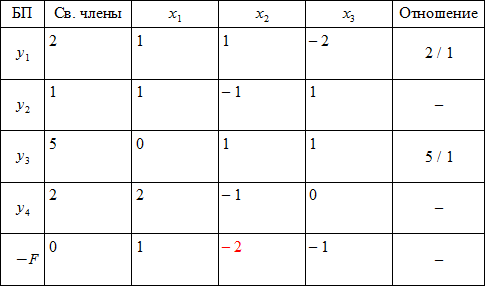
\includegraphics[width=0.7\linewidth]{lp_find_optsol_1.png}}
\caption{Начальная симплекс-таблица для поиска оптимального решения}
\label{fig:lp_find_optsol_1}
\end{figure}

Выбираем в качестве разрешающей строки ту, где найденное выше отношение минимально; на пересечении разрешающей строки и разрешающего столбца определяем разрешающий элемент и находим его обратную величину $\lambda$ (рис. \ref{fig:lp_find_optsol_2}).

\begin{figure}[ht]
\center{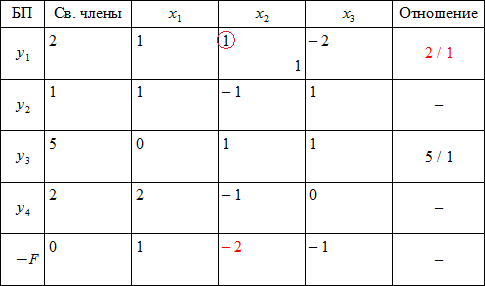
\includegraphics[width=0.7\linewidth]{lp_find_optsol_2.png}}
\caption{Выбор разрешающего элемента}
\label{fig:lp_find_optsol_2}
\end{figure}

\newpage

Делаем замену соответствующих переменных, в результате чего получаем новую симплекс-таблицу (рис. \ref{fig:lp_find_optsol_3} - \ref{fig:lp_find_optsol_5}).

\begin{figure}[ht]
\center{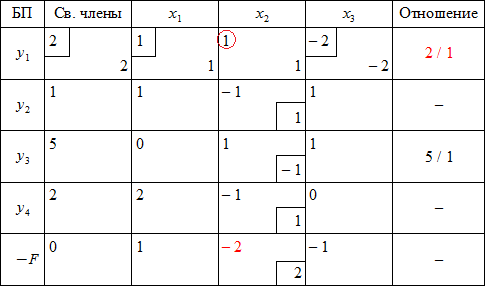
\includegraphics[width=0.7\linewidth]{lp_find_optsol_3.png}}
\caption{Замена $x_{2} \Leftrightarrow y_{1}$, шаг 1}
\label{fig:lp_find_optsol_3}
\end{figure}

\newpage

\begin{figure}[ht]
\center{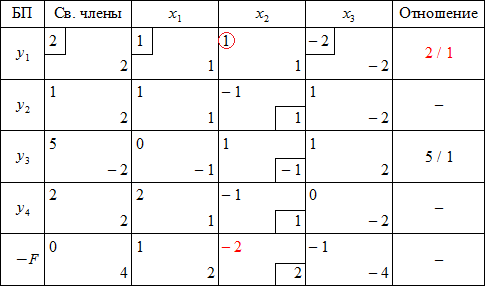
\includegraphics[width=0.7\linewidth]{lp_find_optsol_4.png}}
\caption{Замена $x_{2} \Leftrightarrow y_{1}$, шаг 2}
\label{fig:lp_find_optsol_4}
\end{figure}

\begin{figure}[ht]
\center{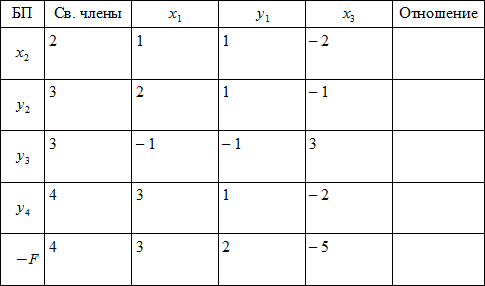
\includegraphics[width=0.7\linewidth]{lp_find_optsol_5.png}}
\caption{Замена $x_{2} \Leftrightarrow y_{1}$, шаг 3}
\label{fig:lp_find_optsol_5}
\end{figure}

Видно, что отрицательный коэффициент, от которого мы хотели избавиться, стал положительным. Выполнив все описанные выше действия для избавления от оставшегося отрицательного коэффициента, получим симплекс-таблицу, в которой все коэффициенты при свободных переменных в линейной форме неотрицательны (рис. \ref{fig:lp_find_optsol_6}).

\newpage

\begin{figure}[ht]
\center{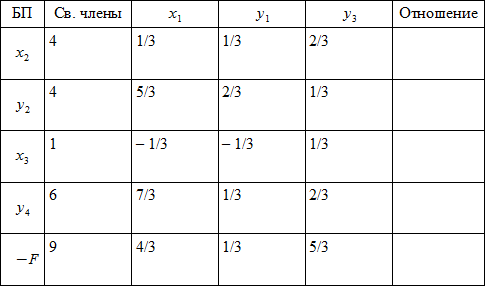
\includegraphics[width=0.7\linewidth]{lp_find_optsol_6.png}}
\caption{Итоговая симплекс-таблица}
\label{fig:lp_find_optsol_6}
\end{figure}

В результате находим решение $(x_{1}, x_{2}, x_{3}, y_{1}, y_{2}, y_{3}, y_{4})^{T} = (0, 4, 1, 0, 4, 0, 6)^{T}$ и минимальное значение линейной формы $-F = 9 \Rightarrow F = -9$.

\subsection{Общий алгоритм решения ОЗЛП}
Подробно рассмотрев ход решения ОЗЛП, можно сформулировать общий алгоритм:
\begin{enumerate}
\item Привести ОЗЛП к стандартному виду:
\begin{itemize}
\item выделить свободные и базисные переменные;
\item выразить линейную форму и базисные переменные через свободные переменные;
\item переписать полученные уравнения в стандартном виде для записи в симплекс-таблицу.
\end{itemize}
\item Удостовериться, что при выбранных свободных и базисных переменных есть опорное решение; если это не так, осуществить поиск допустимого опорного решения (см. раздел \ref{sec:search_op_sol});
\item Если в п. 2 удалось найти допустимое опорное решение, проверить его на оптимальность; если оно неоптимально, осуществить поиск оптимального решения (см. раздел \ref{sec:search_opt_sol}).
\end{enumerate}

Помимо нахождения непосредственно оптимального решения, данный алгоритм позволяет выявить особые случаи, встречающиеся при решении ОЗЛП (см. раздел \ref{sec:ozlp_spec_prop}):
\begin{enumerate}
\item Бесконечное множество решений. Выявляется при наличии нулевых коэффициентов в строке <<$-F$>> после нахождения оптимального решения.
\item ОДР не ограничена. Выявляется на этапе поиска оптимального решения, когда невозможно выбрать разрешающую строку в симплекс-таблице.
\item Система ограничений несовместна. Выявляется на этапе поиска допустимого опорного решения, когда невозможно выбрать разрешающий столбец.
\end{enumerate}

\section{Решение общей задачи ЛП. Метод искусственного базиса}
В общей задаче ЛП помимо ограничений-равенств есть ограничения-неравенства. Для перехода от общей задачи ЛП к основной задаче ЛП неравенства превращают в равенства добавлением дополнительных переменных:
\begin{equation*}
a_{i1}x_{1} + a_{i2}x_{2} + \ldots + a_{in}x_{n} \leq b_{i} \Leftrightarrow a_{i1}x_{1} + a_{i2}x_{2} + \ldots + a_{in}x_{n} + x_{n+1} = b_{i},\ x_{n+1} \geq 0
\end{equation*}
\begin{equation*}
a_{i1}x_{1} + a_{i2}x_{2} + \ldots + a_{in}x_{n} \geq b_{i} \Leftrightarrow a_{i1}x_{1} + a_{i2}x_{2} + \ldots + a_{in}x_{n} - x_{n+1} = b_{i},\ x_{n+1} \geq 0
\end{equation*}

Хотелось бы вводить эти дополнительные переменные таким образом, чтобы получившаяся в результате система ограничений-равенств позволяла бы легко выбрать базис для построения исходной симплекс-таблицы. Для этого предназначен метод искусственного базиса.

Метод состоит в том, что после добавления дополнительных переменных для перехода от неравенств к равенствам, в систему ограничений вводятся \textbf{вспомогательные} (или \textbf{искусственные}) переменные $r_{i}$ согласно следующему правилу: по одной искусственной переменной добавляется со знаком <<+>> в те ограничения, которые в исходной системе имели тип <<=>> или <<$\geq$>>.

Несмотря на то, что и дополнительные, и вспомогательные переменные создаются искусственно и используются для создания исходного базиса, их значения в решении сильно отличаются:
\begin{itemize}
\item дополнительные переменные сообщают, насколько соответствующее им ограничение <<недоиспользовано>>. Значение дополнительной переменной, равное нулю, соответствует равенству значений правых и левых частей ограничения;
\item вспомогательные переменные сообщают, насколько данное условие далеко от допустимого (относительно конкретного ограничения). Если значение вспомогательной переменной больше нуля, то данное решение не выполняет определенное ограничение, а значит, не является допустимым.
\end{itemize}

Иными словами, ненулевое значение дополнительной переменной может (но не должно) сигнализировать о \textit{неоптимальности} решения. Ненулевое значение вспомогательной переменной сигнализирует о \textit{недопустимости} решения.

В линейную форму искусственные переменные вводятся с коэффициентом $M \gg 1$, который имеет смысл <<штрафа>> за введение искусственных переменных. В случае задачи минимизации искусственные переменные прибавляются к функции цели, в случае задачи максимизации - вычитаются:
\begin{equation*}
F = c_{1}x_{1} + c_{2}x_{2} + \ldots + c_{n}x_{n} + M(r_{1} + r_{2} + \ldots + r_{k}) \rightarrow \min
\end{equation*}
\begin{equation*}
F = c_{1}x_{1} + c_{2}x_{2} + \ldots + c_{n}x_{n} - M(r_{1} + r_{2} + \ldots + r_{k}) \rightarrow \max
\end{equation*}

Для отражения этого факта в симплекс-таблицу вводится еще одна строка, которая соответствует так называемой <<M-функции>>. Чтобы определить коэффициенты для этой строки, необходимо просуммировать коэффициенты строк, соответствующих искусственным переменным, и результат взять с обратным знаком. 

После этого начинается обмен свободных и базисных переменных, причем разрешающий столбец на каждой итерации определяется по <<М-строке>> следующим образом: выбирается тот столбец, где значение коэффициента отрицательно и максимально по модулю. Разрешающая строка выбирается так же, как и в обычном симплекс-методе, за исключением того, что рассматриваются только строки, соответствующие искусственным переменным.

Таким образом, из базиса постепенно выводятся все искусственные переменные. После того, как искусственная переменная выведена из базиса, соответствующий ей столбец можно вычеркнуть из симплекс-таблицы. Если все искусственные переменные удалось вывести из базиса (и, соответственно, убрать их из симплекс-таблицы), то найдено допустимое опорное решение и далее следует искать оптимальное решение, как это изложено в разделе \ref{sec:search_opt_sol}. Если же хотя бы одну искусственную переменную не удалось вывести из базиса, то задача ЛП не имеет решения.

\clearpage

\chapter{Комбинаторная оптимизация}

\clearpage

\chapter{Стохастическая оптимизация}

\clearpage

\addcontentsline{toc}{chapter}{Литература} % список литературы автоматически в оглавление не попадает
\bibliography{biblio/doc}

\end{document}